\documentclass[10pt]{article}
\usepackage[margin=0.8in]{geometry}
\usepackage{amsmath,amssymb,booktabs,longtable,pdflscape,array,hyperref,braket,graphicx,placeins}
\usepackage[numbers,sort&compress]{natbib}
\setlength{\emergencystretch}{2em}
\hypersetup{colorlinks=true,linkcolor=black,urlcolor=blue,hypertexnames=false}
\newcommand{\suppsection}[1]{\section*{#1}}
\newcolumntype{P}[1]{>{\raggedright\arraybackslash}p{#1}}
\newtheorem{proposition}{Proposition}
\newtheorem{corollary}[proposition]{Corollary}
\renewcommand{\theproposition}{S\arabic{proposition}}
\renewcommand{\theequation}{S\arabic{equation}}
\renewcommand{\thefigure}{S\arabic{figure}}
\renewcommand{\thetable}{S\arabic{table}}
\begin{document}
\begin{center}
{\Large\bfseries Supplemental Material for}\\[0.6em]
{\large\bfseries Finite-Instance Resource Certification for Group-Conditioned Discrimination of Huffman-Shaped Quantum Ensembles}\\[1em]
Songyao Xue and Mengsi Zhang
\end{center}
This supplement gives the frozen matched-comparison protocol, full registered results, stored-certificate validation, and secondary analyses. The matched discrimination evidence in S1--S5 uses the same group side information on both arms. The scalarized, approximate-decoder, and effective-noise analyses in S6--S22 have their own declared comparison conventions.

\suppsection{S1. Frozen registry and evidence provenance}
The analysis registry was frozen before evaluation, at preregistration commit
\begin{center}\small\texttt{830fe5a91348088710b1409de9f4c329d09f5419}.\end{center}
The result commit is \texttt{7607907}. Registry identifier \texttt{PHASE1D-DETERMINISTIC-CYCLIC-001} identifies the deterministic architecture and evaluation matrix. The complete registry, source seeds, package versions, and implementation hashes are in \url{PHASE_1D_REGISTRY.json}. Its SHA-256 digest is
\begin{center}\footnotesize\texttt{5e1a092fef6743380ab828c7ba13a8a1385b87bbc9bc621d9341254484b8c036}.\end{center}
All 220 registered rows are in \url{data/phase1d_registered_results.csv}. Pre-SDP diagnostics, source states, supports, Gram matrices, primal effects, and dual operators are stored with the run manifest. The row-level trace links each result to its source and operator hashes. The registry and original result artifacts are unchanged by table and figure aggregation.

The 40 source entries comprise five seeds for each family and $M=4,8$. Near-uniform sources normalize clipped values $1/M+\xi_i$, with independent seeded Gaussian $\xi_i$ of standard deviation $0.04/M$ and clipping floor $10^{-6}$. Zipf sources have $p_i\propto(i+1)^{-0.8}$. Dirichlet sources have parameter vector $(2,\ldots,2)$. Strong-skew sources have $p_0=0.75$ and equal tail mass. Zipf and strong-skew seed replicas share their prior vectors across seeds. Overall there are 24 distinct priors.

A registered row fixes a source entry, grouping rule, and group count. A source instance is the registered family/$M$/seed entry. A distinct prior is determined by the stored full-precision vector and its hash. A seed replica with the same prior is not an additional independent distribution. The robust-positive rows under G2 correspond to three priors across both alphabet sizes; the E2-positive $M=8,G=2$ subset corresponds to two priors. Counting is deterministic and deduplicated within each reported cell.

\suppsection{S2. Matched encoder and grouping details}
Both arms use $n_{\max}=\max(n_{\rm fix},\max_i l_i^H)+1$, cyclic placement with shift zero, equal-modulus amplitudes, and the same deterministic phase ansatz. At each probability-ordered symbol, the cursor advances by half its support size. The encoder uses the frozen NumPy \texttt{argsort(-p)} ordering, and wrapped supports are sorted by \texttt{unique}. The supplied-length adapter applies the same rules to $l^H$ and the constant fixed-length vector. Source seeds are offset by 100 for the encoder interface, but this deterministic mode makes no random draws and uses zero optimizer iterations. The implementation and configuration hashes accompany the registry.

For G0 all symbols form one group. G1 assigns the zero-based index modulo $G$. G2 sorts by $(-p_i,i)$, then assigns each symbol to the least-probability group, resolving group-mass ties by group index. G3 forms a binary Huffman heap keyed by weight and node identifier: leaves use symbol indices and internal nodes use increasing merge serials. Starting at the root, the cut repeatedly splits the shallowest nonleaf frontier node, resolving ties by its minimum leaf index and then its serial. Final subtrees are ordered by minimum leaf index. These rules fix the same partition on H and F before inspecting quantum geometry.

For each group, the diagnostics store its mass $p_g$, maximum off-diagonal Gram magnitude, and
\begin{equation}
 A_{\mathrm{in},g}^X=\sum_{\substack{i<j\\i,j\in\mathcal G_g}}q_i^{(g)}q_j^{(g)}|\Gamma_{ij}^X|^2.
\end{equation}
Nontriviality requires at least two members and off-diagonal magnitude above $10^{-10}$. E1 requires a common nontrivial group on both arms; E2 requires at least one nonsingleton and nontriviality of every nonsingleton group on both arms. All classifications agree at the sensitivity threshold $10^{-8}$. There are 65 singleton-containing rows and 80 singleton groups, counted over partitions rather than separately for each arm. No eligibility condition removes a row from evaluation.

\suppsection{S3. Conditional SDP formulation and certificate verification}
For each arm $X$ and group $g$, solve
\begin{align}
 P_{X,g}^*&=\max_{\{E_i\}}\sum_{i\in\mathcal G_g}q_i^{(g)}\operatorname{Tr}(E_i\rho_i^X),\\
 &E_i\succeq0,\quad\sum_iE_i=I,\nonumber\\
 D_{X,g}^*&=\min_{Y_g}\operatorname{Tr}Y_g,\quad
 Y_g\succeq q_i^{(g)}\rho_i^X\quad(i\in\mathcal G_g).
\end{align}
The conditional priors sum to one. The aggregate lower and upper bounds are $\sum_gp_g\underline P_{X,g}$ and $\sum_gp_g\overline P_{X,g}$; the matched certificate uses H lower and F upper. The F dual is grouped with the same labels and partition, rather than the global unlabeled dual.

SCS uses tolerance $5\times10^{-6}$, at most 25000 iterations, and a 30-s time limit per solve. State-span compression uses rank threshold $10^{-12}$. Returned effects are Hermitized, projected to their positive parts, regularized, and normalized by the inverse square root of their sum. After lifting, the orthogonal complement is assigned across effects to complete the ambient POVM. The dual is Hermitized, lifted, and shifted using the maximum slack violation and safety shift $5\times10^{-8}$. The full-space check verifies all $Y_g-q_i^{(g)}\rho_i^X\succeq0$ and POVM completeness, with feasibility tolerance $10^{-7}$ and aggregation tolerance $10^{-12}$. Singleton tasks are handled analytically. Both arms' primal and dual objects are stored even though the main certificate uses only H lower and F upper.

The robust-positive threshold is $100(5\times10^{-6})=5\times10^{-4}$. Every registered case is preserved; all 220 resulting cases pass. Independently reconstructing the stored objects checks 1040 conditional certificate sets. Every robust-positive row was repeat-solved, and the independent uncompressed formulation confirmed all eight robust-positive rows. Five Zipf replicas share identical inputs and their full-space crosscheck is cached; there are four distinct encoder/partition pairs among the eight rows. This is floating-point verification with explicit residual checks, not exact-arithmetic or interval certification.

The files \url{data/phase1d_robust_replication.csv} and \url{data/phase1d_fullspace_crosscheck.csv} record the repeat and full-space comparisons. The $M=8,G=2$ G2 priors are the Zipf vector and the seed-2837 Dirichlet vector. Their registered gaps are $0.006090$ and $0.003941$; full-space gaps are $0.006025$ and $0.003776$ after rounding. Full vectors and corresponding states remain in the source archives.

\suppsection{S4. Complete registered results}
The following table includes all 220 rows, without filtering by eligibility, triviality, or certificate sign. Registered seed entries and duplicate priors remain visible. The $M=4$ G2 robust-positive row fails E2; the $M=4$ G3 robust-positive row satisfies E2 but supplies only one prior for that regime. The replicated two-prior E2 evidence occurs in G2 with $M=8,G=2$.
\begin{landscape}\scriptsize
\begin{longtable}{@{}rlrrlrrrrrr@{}}
\caption{All 220 registered rows. Source abbreviations N, Z, D, S denote near-uniform, Zipf, Dirichlet, and strong-skew; rule numbers 0--3 denote G0--G3. T marks a fixed-trivial task, R a robust-positive certificate. All solver/certificate checks passed. Full partitions, priors, residuals, and operator files accompany the CSV.}\label{tab:allrows}\\
\toprule $M$ & Source & Seed & Rule & $G$ & E1 & E2 & T & $\underline P_H$ & $\overline P_F$ & $\Delta_{\rm pair}$ / R \\ \midrule\endfirsthead
\toprule $M$ & Source & Seed & Rule & $G$ & E1 & E2 & T & $\underline P_H$ & $\overline P_F$ & $\Delta_{\rm pair}$ / R \\ \midrule\endhead
\bottomrule\endfoot
4 & N & 3044 & 0 & 1 & 1 & 1 & 0 & 0.882816 & 0.882834 & -0.000019 / 0 \\
4 & N & 3044 & 1 & 2 & 1 & 0 & 0 & 0.966443 & 0.966459 & -0.000016 / 0 \\
4 & N & 3044 & 2 & 2 & 1 & 0 & 0 & 0.966443 & 0.966459 & -0.000016 / 0 \\
4 & N & 3044 & 3 & 2 & 1 & 1 & 0 & 0.933024 & 0.933040 & -0.000016 / 0 \\
4 & N & 3061 & 0 & 1 & 1 & 1 & 0 & 0.882410 & 0.882428 & -0.000018 / 0 \\
4 & N & 3061 & 1 & 2 & 1 & 0 & 0 & 0.966130 & 0.966148 & -0.000018 / 0 \\
4 & N & 3061 & 2 & 2 & 1 & 0 & 0 & 0.966130 & 0.966148 & -0.000018 / 0 \\
4 & N & 3061 & 3 & 2 & 1 & 1 & 0 & 0.933033 & 0.933049 & -0.000016 / 0 \\
4 & N & 3078 & 0 & 1 & 1 & 1 & 0 & 0.882912 & 0.882930 & -0.000018 / 0 \\
4 & N & 3078 & 1 & 2 & 1 & 0 & 0 & 0.966494 & 0.966517 & -0.000022 / 0 \\
4 & N & 3078 & 2 & 2 & 1 & 0 & 0 & 0.966494 & 0.966517 & -0.000022 / 0 \\
4 & N & 3078 & 3 & 2 & 1 & 1 & 0 & 0.933047 & 0.933074 & -0.000028 / 0 \\
4 & N & 3095 & 0 & 1 & 1 & 1 & 0 & 0.883301 & 0.883319 & -0.000019 / 0 \\
4 & N & 3095 & 1 & 2 & 1 & 1 & 0 & 0.933039 & 0.933062 & -0.000023 / 0 \\
4 & N & 3095 & 2 & 2 & 1 & 0 & 0 & 0.966784 & 0.966835 & -0.000051 / 0 \\
4 & N & 3095 & 3 & 2 & 1 & 1 & 0 & 0.933039 & 0.933062 & -0.000023 / 0 \\
4 & N & 3112 & 0 & 1 & 1 & 1 & 0 & 0.882257 & 0.882261 & -0.000003 / 0 \\
4 & N & 3112 & 1 & 2 & 1 & 0 & 0 & 0.965969 & 0.965995 & -0.000026 / 0 \\
4 & N & 3112 & 2 & 2 & 1 & 0 & 0 & 0.965969 & 0.965995 & -0.000026 / 0 \\
4 & N & 3112 & 3 & 2 & 1 & 1 & 0 & 0.933083 & 0.933116 & -0.000033 / 0 \\
4 & Z & 51408 & 0 & 1 & 1 & 1 & 0 & 0.927644 & 0.937417 & -0.009774 / 0 \\
4 & Z & 51408 & 1 & 2 & 0 & 0 & 1 & 0.959023 & 1.000024 & -0.041001 / 0 \\
4 & Z & 51408 & 2 & 2 & 1 & 1 & 0 & 0.961127 & 0.966974 & -0.005847 / 0 \\
4 & Z & 51408 & 3 & 2 & 1 & 1 & 0 & 0.961127 & 0.966974 & -0.005847 / 0 \\
4 & Z & 51425 & 0 & 1 & 1 & 1 & 0 & 0.927644 & 0.937417 & -0.009774 / 0 \\
4 & Z & 51425 & 1 & 2 & 0 & 0 & 1 & 0.959023 & 1.000024 & -0.041001 / 0 \\
4 & Z & 51425 & 2 & 2 & 1 & 1 & 0 & 0.961127 & 0.966974 & -0.005847 / 0 \\
4 & Z & 51425 & 3 & 2 & 1 & 1 & 0 & 0.961127 & 0.966974 & -0.005847 / 0 \\
4 & Z & 51442 & 0 & 1 & 1 & 1 & 0 & 0.927644 & 0.937417 & -0.009774 / 0 \\
4 & Z & 51442 & 1 & 2 & 0 & 0 & 1 & 0.959023 & 1.000024 & -0.041001 / 0 \\
4 & Z & 51442 & 2 & 2 & 1 & 1 & 0 & 0.961127 & 0.966974 & -0.005847 / 0 \\
4 & Z & 51442 & 3 & 2 & 1 & 1 & 0 & 0.961127 & 0.966974 & -0.005847 / 0 \\
4 & Z & 51459 & 0 & 1 & 1 & 1 & 0 & 0.927644 & 0.937417 & -0.009774 / 0 \\
4 & Z & 51459 & 1 & 2 & 0 & 0 & 1 & 0.959023 & 1.000024 & -0.041001 / 0 \\
4 & Z & 51459 & 2 & 2 & 1 & 1 & 0 & 0.961127 & 0.966974 & -0.005847 / 0 \\
4 & Z & 51459 & 3 & 2 & 1 & 1 & 0 & 0.961127 & 0.966974 & -0.005847 / 0 \\
4 & Z & 51476 & 0 & 1 & 1 & 1 & 0 & 0.927644 & 0.937417 & -0.009774 / 0 \\
4 & Z & 51476 & 1 & 2 & 0 & 0 & 1 & 0.959023 & 1.000024 & -0.041001 / 0 \\
4 & Z & 51476 & 2 & 2 & 1 & 1 & 0 & 0.961127 & 0.966974 & -0.005847 / 0 \\
4 & Z & 51476 & 3 & 2 & 1 & 1 & 0 & 0.961127 & 0.966974 & -0.005847 / 0 \\
4 & D & 2420 & 0 & 1 & 1 & 1 & 0 & 0.934926 & 0.974883 & -0.039957 / 0 \\
4 & D & 2420 & 1 & 2 & 1 & 0 & 0 & 0.977921 & 0.998158 & -0.020238 / 0 \\
4 & D & 2420 & 2 & 2 & 1 & 1 & 0 & 0.966066 & 0.997091 & -0.031025 / 0 \\
4 & D & 2420 & 3 & 2 & 1 & 1 & 0 & 0.966066 & 0.997091 & -0.031025 / 0 \\
4 & D & 2437 & 0 & 1 & 1 & 1 & 0 & 0.862380 & 0.991697 & -0.129318 / 0 \\
4 & D & 2437 & 1 & 2 & 1 & 1 & 0 & 0.947576 & 0.994339 & -0.046764 / 0 \\
4 & D & 2437 & 2 & 2 & 1 & 0 & 0 & 0.943643 & 0.997482 & -0.053839 / 0 \\
4 & D & 2437 & 3 & 2 & 1 & 1 & 0 & 0.924992 & 0.995505 & -0.070514 / 0 \\
4 & D & 2454 & 0 & 1 & 1 & 1 & 0 & 0.887723 & 0.962533 & -0.074810 / 0 \\
4 & D & 2454 & 1 & 2 & 0 & 0 & 1 & 0.955782 & 1.000001 & -0.044219 / 0 \\
4 & D & 2454 & 2 & 2 & 1 & 0 & 0 & 0.948474 & 0.977234 & -0.028760 / 0 \\
4 & D & 2454 & 3 & 2 & 1 & 1 & 0 & 0.934481 & 0.966717 & -0.032236 / 0 \\
4 & D & 2471 & 0 & 1 & 1 & 1 & 0 & 0.945174 & 0.991884 & -0.046709 / 0 \\
4 & D & 2471 & 1 & 2 & 1 & 1 & 0 & 0.984494 & 0.994767 & -0.010273 / 0 \\
4 & D & 2471 & 2 & 2 & 1 & 0 & 0 & 0.996195 & 0.997401 & -0.001206 / 0 \\
4 & D & 2471 & 3 & 2 & 1 & 1 & 0 & 0.981435 & 0.996254 & -0.014819 / 0 \\
4 & D & 2488 & 0 & 1 & 1 & 1 & 0 & 0.940146 & 0.972018 & -0.031872 / 0 \\
4 & D & 2488 & 1 & 2 & 1 & 1 & 0 & 0.955128 & 0.994825 & -0.039697 / 0 \\
4 & D & 2488 & 2 & 2 & 1 & 0 & 0 & 0.997244 & 0.977851 & 0.019392 / 1 \\
4 & D & 2488 & 3 & 2 & 1 & 1 & 0 & 0.987221 & 0.976963 & 0.010257 / 1 \\
4 & S & 4115 & 0 & 1 & 1 & 1 & 0 & 0.958782 & 0.971593 & -0.012811 / 0 \\
4 & S & 4115 & 1 & 2 & 0 & 0 & 1 & 0.983100 & 1.000039 & -0.016939 / 0 \\
4 & S & 4115 & 2 & 2 & 1 & 1 & 0 & 0.982443 & 0.984934 & -0.002491 / 0 \\
4 & S & 4115 & 3 & 2 & 1 & 1 & 0 & 0.982443 & 0.984934 & -0.002491 / 0 \\
4 & S & 4132 & 0 & 1 & 1 & 1 & 0 & 0.958782 & 0.971593 & -0.012811 / 0 \\
4 & S & 4132 & 1 & 2 & 0 & 0 & 1 & 0.983100 & 1.000039 & -0.016939 / 0 \\
4 & S & 4132 & 2 & 2 & 1 & 1 & 0 & 0.982443 & 0.984934 & -0.002491 / 0 \\
4 & S & 4132 & 3 & 2 & 1 & 1 & 0 & 0.982443 & 0.984934 & -0.002491 / 0 \\
4 & S & 4149 & 0 & 1 & 1 & 1 & 0 & 0.958782 & 0.971593 & -0.012811 / 0 \\
4 & S & 4149 & 1 & 2 & 0 & 0 & 1 & 0.983100 & 1.000039 & -0.016939 / 0 \\
4 & S & 4149 & 2 & 2 & 1 & 1 & 0 & 0.982443 & 0.984934 & -0.002491 / 0 \\
4 & S & 4149 & 3 & 2 & 1 & 1 & 0 & 0.982443 & 0.984934 & -0.002491 / 0 \\
4 & S & 4166 & 0 & 1 & 1 & 1 & 0 & 0.958782 & 0.971593 & -0.012811 / 0 \\
4 & S & 4166 & 1 & 2 & 0 & 0 & 1 & 0.983100 & 1.000039 & -0.016939 / 0 \\
4 & S & 4166 & 2 & 2 & 1 & 1 & 0 & 0.982443 & 0.984934 & -0.002491 / 0 \\
4 & S & 4166 & 3 & 2 & 1 & 1 & 0 & 0.982443 & 0.984934 & -0.002491 / 0 \\
4 & S & 4183 & 0 & 1 & 1 & 1 & 0 & 0.958782 & 0.971593 & -0.012811 / 0 \\
4 & S & 4183 & 1 & 2 & 0 & 0 & 1 & 0.983100 & 1.000039 & -0.016939 / 0 \\
4 & S & 4183 & 2 & 2 & 1 & 1 & 0 & 0.982443 & 0.984934 & -0.002491 / 0 \\
4 & S & 4183 & 3 & 2 & 1 & 1 & 0 & 0.982443 & 0.984934 & -0.002491 / 0 \\
8 & N & 3084 & 0 & 1 & 1 & 1 & 0 & 0.850773 & 0.850775 & -0.000002 / 0 \\
8 & N & 3084 & 1 & 2 & 1 & 1 & 0 & 0.926326 & 0.926337 & -0.000010 / 0 \\
8 & N & 3084 & 1 & 4 & 1 & 0 & 0 & 0.983116 & 0.983160 & -0.000044 / 0 \\
8 & N & 3084 & 2 & 2 & 1 & 0 & 0 & 0.983114 & 0.983171 & -0.000057 / 0 \\
8 & N & 3084 & 2 & 4 & 1 & 0 & 0 & 0.983213 & 0.983227 & -0.000014 / 0 \\
8 & N & 3084 & 3 & 2 & 1 & 1 & 0 & 0.883278 & 0.883312 & -0.000033 / 0 \\
8 & N & 3084 & 3 & 4 & 1 & 1 & 0 & 0.933047 & 0.933086 & -0.000039 / 0 \\
8 & N & 3101 & 0 & 1 & 1 & 1 & 0 & 0.850139 & 0.850141 & -0.000002 / 0 \\
8 & N & 3101 & 1 & 2 & 1 & 1 & 0 & 0.949583 & 0.949608 & -0.000025 / 0 \\
8 & N & 3101 & 1 & 4 & 0 & 0 & 1 & 1.000000 & 1.000034 & -0.000034 / 0 \\
8 & N & 3101 & 2 & 2 & 1 & 1 & 0 & 0.966015 & 0.966019 & -0.000004 / 0 \\
8 & N & 3101 & 2 & 4 & 1 & 0 & 0 & 0.983175 & 0.983210 & -0.000035 / 0 \\
8 & N & 3101 & 3 & 2 & 1 & 1 & 0 & 0.882759 & 0.882796 & -0.000037 / 0 \\
8 & N & 3101 & 3 & 4 & 1 & 1 & 0 & 0.933014 & 0.933025 & -0.000011 / 0 \\
8 & N & 3118 & 0 & 1 & 1 & 1 & 0 & 0.850424 & 0.850426 & -0.000002 / 0 \\
8 & N & 3118 & 1 & 2 & 1 & 0 & 0 & 0.983608 & 0.983655 & -0.000047 / 0 \\
8 & N & 3118 & 1 & 4 & 0 & 0 & 1 & 1.000000 & 1.000031 & -0.000031 / 0 \\
8 & N & 3118 & 2 & 2 & 1 & 1 & 0 & 0.966539 & 0.966607 & -0.000068 / 0 \\
8 & N & 3118 & 2 & 4 & 1 & 0 & 0 & 0.983217 & 0.983249 & -0.000033 / 0 \\
8 & N & 3118 & 3 & 2 & 1 & 1 & 0 & 0.882935 & 0.882973 & -0.000037 / 0 \\
8 & N & 3118 & 3 & 4 & 1 & 1 & 0 & 0.933013 & 0.933018 & -0.000005 / 0 \\
8 & N & 3135 & 0 & 1 & 1 & 1 & 0 & 0.850575 & 0.850577 & -0.000002 / 0 \\
8 & N & 3135 & 1 & 2 & 1 & 0 & 0 & 0.983364 & 0.983384 & -0.000020 / 0 \\
8 & N & 3135 & 1 & 4 & 0 & 0 & 1 & 1.000000 & 1.000044 & -0.000044 / 0 \\
8 & N & 3135 & 2 & 2 & 1 & 1 & 0 & 0.966127 & 0.966146 & -0.000019 / 0 \\
8 & N & 3135 & 2 & 4 & 1 & 0 & 0 & 0.983367 & 0.983414 & -0.000048 / 0 \\
8 & N & 3135 & 3 & 2 & 1 & 1 & 0 & 0.882842 & 0.882879 & -0.000037 / 0 \\
8 & N & 3135 & 3 & 4 & 1 & 1 & 0 & 0.933013 & 0.933020 & -0.000007 / 0 \\
8 & N & 3152 & 0 & 1 & 1 & 1 & 0 & 0.850758 & 0.850760 & -0.000002 / 0 \\
8 & N & 3152 & 1 & 2 & 1 & 1 & 0 & 0.967050 & 0.967054 & -0.000004 / 0 \\
8 & N & 3152 & 1 & 4 & 1 & 0 & 0 & 0.983148 & 0.983197 & -0.000049 / 0 \\
8 & N & 3152 & 2 & 2 & 1 & 1 & 0 & 0.966818 & 0.966823 & -0.000005 / 0 \\
8 & N & 3152 & 2 & 4 & 1 & 0 & 0 & 0.983148 & 0.983197 & -0.000049 / 0 \\
8 & N & 3152 & 3 & 2 & 1 & 1 & 0 & 0.883325 & 0.883361 & -0.000036 / 0 \\
8 & N & 3152 & 3 & 4 & 1 & 1 & 0 & 0.933026 & 0.933053 & -0.000026 / 0 \\
8 & Z & 51808 & 0 & 1 & 1 & 1 & 0 & 0.909052 & 0.925163 & -0.016111 / 0 \\
8 & Z & 51808 & 1 & 2 & 0 & 0 & 1 & 0.993973 & 1.000004 & -0.006030 / 0 \\
8 & Z & 51808 & 1 & 4 & 0 & 0 & 1 & 0.999999 & 1.000022 & -0.000023 / 0 \\
8 & Z & 51808 & 2 & 2 & 1 & 1 & 0 & 0.975660 & 0.969570 & 0.006090 / 1 \\
8 & Z & 51808 & 2 & 4 & 1 & 0 & 0 & 0.978038 & 0.992089 & -0.014051 / 0 \\
8 & Z & 51808 & 3 & 2 & 1 & 1 & 0 & 0.980664 & 0.987972 & -0.007307 / 0 \\
8 & Z & 51808 & 3 & 4 & 1 & 1 & 0 & 0.981137 & 0.987971 & -0.006835 / 0 \\
8 & Z & 51825 & 0 & 1 & 1 & 1 & 0 & 0.909052 & 0.925163 & -0.016111 / 0 \\
8 & Z & 51825 & 1 & 2 & 0 & 0 & 1 & 0.993973 & 1.000004 & -0.006030 / 0 \\
8 & Z & 51825 & 1 & 4 & 0 & 0 & 1 & 0.999999 & 1.000022 & -0.000023 / 0 \\
8 & Z & 51825 & 2 & 2 & 1 & 1 & 0 & 0.975660 & 0.969570 & 0.006090 / 1 \\
8 & Z & 51825 & 2 & 4 & 1 & 0 & 0 & 0.978038 & 0.992089 & -0.014051 / 0 \\
8 & Z & 51825 & 3 & 2 & 1 & 1 & 0 & 0.980664 & 0.987972 & -0.007307 / 0 \\
8 & Z & 51825 & 3 & 4 & 1 & 1 & 0 & 0.981137 & 0.987971 & -0.006835 / 0 \\
8 & Z & 51842 & 0 & 1 & 1 & 1 & 0 & 0.909052 & 0.925163 & -0.016111 / 0 \\
8 & Z & 51842 & 1 & 2 & 0 & 0 & 1 & 0.993973 & 1.000004 & -0.006030 / 0 \\
8 & Z & 51842 & 1 & 4 & 0 & 0 & 1 & 0.999999 & 1.000022 & -0.000023 / 0 \\
8 & Z & 51842 & 2 & 2 & 1 & 1 & 0 & 0.975660 & 0.969570 & 0.006090 / 1 \\
8 & Z & 51842 & 2 & 4 & 1 & 0 & 0 & 0.978038 & 0.992089 & -0.014051 / 0 \\
8 & Z & 51842 & 3 & 2 & 1 & 1 & 0 & 0.980664 & 0.987972 & -0.007307 / 0 \\
8 & Z & 51842 & 3 & 4 & 1 & 1 & 0 & 0.981137 & 0.987971 & -0.006835 / 0 \\
8 & Z & 51859 & 0 & 1 & 1 & 1 & 0 & 0.909052 & 0.925163 & -0.016111 / 0 \\
8 & Z & 51859 & 1 & 2 & 0 & 0 & 1 & 0.993973 & 1.000004 & -0.006030 / 0 \\
8 & Z & 51859 & 1 & 4 & 0 & 0 & 1 & 0.999999 & 1.000022 & -0.000023 / 0 \\
8 & Z & 51859 & 2 & 2 & 1 & 1 & 0 & 0.975660 & 0.969570 & 0.006090 / 1 \\
8 & Z & 51859 & 2 & 4 & 1 & 0 & 0 & 0.978038 & 0.992089 & -0.014051 / 0 \\
8 & Z & 51859 & 3 & 2 & 1 & 1 & 0 & 0.980664 & 0.987972 & -0.007307 / 0 \\
8 & Z & 51859 & 3 & 4 & 1 & 1 & 0 & 0.981137 & 0.987971 & -0.006835 / 0 \\
8 & Z & 51876 & 0 & 1 & 1 & 1 & 0 & 0.909052 & 0.925163 & -0.016111 / 0 \\
8 & Z & 51876 & 1 & 2 & 0 & 0 & 1 & 0.993973 & 1.000004 & -0.006030 / 0 \\
8 & Z & 51876 & 1 & 4 & 0 & 0 & 1 & 0.999999 & 1.000022 & -0.000023 / 0 \\
8 & Z & 51876 & 2 & 2 & 1 & 1 & 0 & 0.975660 & 0.969570 & 0.006090 / 1 \\
8 & Z & 51876 & 2 & 4 & 1 & 0 & 0 & 0.978038 & 0.992089 & -0.014051 / 0 \\
8 & Z & 51876 & 3 & 2 & 1 & 1 & 0 & 0.980664 & 0.987972 & -0.007307 / 0 \\
8 & Z & 51876 & 3 & 4 & 1 & 1 & 0 & 0.981137 & 0.987971 & -0.006835 / 0 \\
8 & D & 2820 & 0 & 1 & 1 & 1 & 0 & 0.890449 & 0.927765 & -0.037316 / 0 \\
8 & D & 2820 & 1 & 2 & 1 & 1 & 0 & 0.966035 & 0.980276 & -0.014241 / 0 \\
8 & D & 2820 & 1 & 4 & 1 & 0 & 0 & 0.970510 & 0.981941 & -0.011431 / 0 \\
8 & D & 2820 & 2 & 2 & 1 & 0 & 0 & 0.983441 & 0.986320 & -0.002879 / 0 \\
8 & D & 2820 & 2 & 4 & 1 & 0 & 0 & 0.985908 & 0.985953 & -0.000045 / 0 \\
8 & D & 2820 & 3 & 2 & 1 & 1 & 0 & 0.892780 & 0.929989 & -0.037208 / 0 \\
8 & D & 2820 & 3 & 4 & 1 & 1 & 0 & 0.973062 & 0.978331 & -0.005269 / 0 \\
8 & D & 2837 & 0 & 1 & 1 & 1 & 0 & 0.956324 & 0.981278 & -0.024954 / 0 \\
8 & D & 2837 & 1 & 2 & 1 & 1 & 0 & 0.982802 & 0.999669 & -0.016867 / 0 \\
8 & D & 2837 & 1 & 4 & 0 & 0 & 1 & 0.989576 & 1.000112 & -0.010536 / 0 \\
8 & D & 2837 & 2 & 2 & 1 & 1 & 0 & 0.991066 & 0.987125 & 0.003941 / 1 \\
8 & D & 2837 & 2 & 4 & 1 & 0 & 0 & 0.995665 & 0.999783 & -0.004118 / 0 \\
8 & D & 2837 & 3 & 2 & 1 & 1 & 0 & 0.978494 & 0.998033 & -0.019539 / 0 \\
8 & D & 2837 & 3 & 4 & 1 & 1 & 0 & 0.987833 & 0.997746 & -0.009913 / 0 \\
8 & D & 2854 & 0 & 1 & 1 & 1 & 0 & 0.957652 & 0.976427 & -0.018775 / 0 \\
8 & D & 2854 & 1 & 2 & 1 & 1 & 0 & 0.994751 & 0.999720 & -0.004969 / 0 \\
8 & D & 2854 & 1 & 4 & 1 & 0 & 0 & 0.994762 & 0.999877 & -0.005115 / 0 \\
8 & D & 2854 & 2 & 2 & 1 & 0 & 0 & 0.990670 & 0.999507 & -0.008837 / 0 \\
8 & D & 2854 & 2 & 4 & 1 & 0 & 0 & 0.993931 & 0.994188 & -0.000257 / 0 \\
8 & D & 2854 & 3 & 2 & 1 & 1 & 0 & 0.977220 & 0.993614 & -0.016394 / 0 \\
8 & D & 2854 & 3 & 4 & 1 & 1 & 0 & 0.977224 & 0.993703 & -0.016479 / 0 \\
8 & D & 2871 & 0 & 1 & 1 & 1 & 0 & 0.951170 & 0.980715 & -0.029545 / 0 \\
8 & D & 2871 & 1 & 2 & 1 & 1 & 0 & 0.983606 & 0.998963 & -0.015357 / 0 \\
8 & D & 2871 & 1 & 4 & 1 & 0 & 0 & 0.995279 & 0.999652 & -0.004372 / 0 \\
8 & D & 2871 & 2 & 2 & 1 & 0 & 0 & 0.994969 & 0.999567 & -0.004598 / 0 \\
8 & D & 2871 & 2 & 4 & 1 & 0 & 0 & 0.994476 & 0.999497 & -0.005021 / 0 \\
8 & D & 2871 & 3 & 2 & 1 & 1 & 0 & 0.963410 & 0.981287 & -0.017877 / 0 \\
8 & D & 2871 & 3 & 4 & 1 & 1 & 0 & 0.978491 & 0.995173 & -0.016681 / 0 \\
8 & D & 2888 & 0 & 1 & 1 & 1 & 0 & 0.893329 & 0.970289 & -0.076960 / 0 \\
8 & D & 2888 & 1 & 2 & 1 & 1 & 0 & 0.918842 & 0.986059 & -0.067217 / 0 \\
8 & D & 2888 & 1 & 4 & 0 & 0 & 1 & 0.997991 & 1.000112 & -0.002121 / 0 \\
8 & D & 2888 & 2 & 2 & 1 & 0 & 0 & 0.947231 & 0.997894 & -0.050663 / 0 \\
8 & D & 2888 & 2 & 4 & 1 & 0 & 0 & 0.979868 & 0.985036 & -0.005168 / 0 \\
8 & D & 2888 & 3 & 2 & 1 & 1 & 0 & 0.940564 & 0.972607 & -0.032042 / 0 \\
8 & D & 2888 & 3 & 4 & 1 & 1 & 0 & 0.981946 & 0.998444 & -0.016498 / 0 \\
8 & S & 4155 & 0 & 1 & 1 & 1 & 0 & 0.954584 & 0.973647 & -0.019063 / 0 \\
8 & S & 4155 & 1 & 2 & 0 & 0 & 1 & 0.993402 & 1.000028 & -0.006626 / 0 \\
8 & S & 4155 & 1 & 4 & 0 & 0 & 1 & 0.999528 & 1.000002 & -0.000474 / 0 \\
8 & S & 4155 & 2 & 2 & 1 & 1 & 0 & 0.967366 & 0.979605 & -0.012239 / 0 \\
8 & S & 4155 & 2 & 4 & 0 & 0 & 1 & 1.000000 & 1.000002 & -0.000002 / 0 \\
8 & S & 4155 & 3 & 2 & 1 & 1 & 0 & 0.967366 & 0.979605 & -0.012239 / 0 \\
8 & S & 4155 & 3 & 4 & 1 & 1 & 0 & 0.978485 & 0.987020 & -0.008536 / 0 \\
8 & S & 4172 & 0 & 1 & 1 & 1 & 0 & 0.954584 & 0.973647 & -0.019063 / 0 \\
8 & S & 4172 & 1 & 2 & 0 & 0 & 1 & 0.993402 & 1.000028 & -0.006626 / 0 \\
8 & S & 4172 & 1 & 4 & 0 & 0 & 1 & 0.999528 & 1.000002 & -0.000474 / 0 \\
8 & S & 4172 & 2 & 2 & 1 & 1 & 0 & 0.967366 & 0.979605 & -0.012239 / 0 \\
8 & S & 4172 & 2 & 4 & 0 & 0 & 1 & 1.000000 & 1.000002 & -0.000002 / 0 \\
8 & S & 4172 & 3 & 2 & 1 & 1 & 0 & 0.967366 & 0.979605 & -0.012239 / 0 \\
8 & S & 4172 & 3 & 4 & 1 & 1 & 0 & 0.978485 & 0.987020 & -0.008536 / 0 \\
8 & S & 4189 & 0 & 1 & 1 & 1 & 0 & 0.954584 & 0.973647 & -0.019063 / 0 \\
8 & S & 4189 & 1 & 2 & 0 & 0 & 1 & 0.993402 & 1.000028 & -0.006626 / 0 \\
8 & S & 4189 & 1 & 4 & 0 & 0 & 1 & 0.999528 & 1.000002 & -0.000474 / 0 \\
8 & S & 4189 & 2 & 2 & 1 & 1 & 0 & 0.967366 & 0.979605 & -0.012239 / 0 \\
8 & S & 4189 & 2 & 4 & 0 & 0 & 1 & 1.000000 & 1.000002 & -0.000002 / 0 \\
8 & S & 4189 & 3 & 2 & 1 & 1 & 0 & 0.967366 & 0.979605 & -0.012239 / 0 \\
8 & S & 4189 & 3 & 4 & 1 & 1 & 0 & 0.978485 & 0.987020 & -0.008536 / 0 \\
8 & S & 4206 & 0 & 1 & 1 & 1 & 0 & 0.954584 & 0.973647 & -0.019063 / 0 \\
8 & S & 4206 & 1 & 2 & 0 & 0 & 1 & 0.993402 & 1.000028 & -0.006626 / 0 \\
8 & S & 4206 & 1 & 4 & 0 & 0 & 1 & 0.999528 & 1.000002 & -0.000474 / 0 \\
8 & S & 4206 & 2 & 2 & 1 & 1 & 0 & 0.967366 & 0.979605 & -0.012239 / 0 \\
8 & S & 4206 & 2 & 4 & 0 & 0 & 1 & 1.000000 & 1.000002 & -0.000002 / 0 \\
8 & S & 4206 & 3 & 2 & 1 & 1 & 0 & 0.967366 & 0.979605 & -0.012239 / 0 \\
8 & S & 4206 & 3 & 4 & 1 & 1 & 0 & 0.978485 & 0.987020 & -0.008536 / 0 \\
8 & S & 4223 & 0 & 1 & 1 & 1 & 0 & 0.954584 & 0.973647 & -0.019063 / 0 \\
8 & S & 4223 & 1 & 2 & 0 & 0 & 1 & 0.993402 & 1.000028 & -0.006626 / 0 \\
8 & S & 4223 & 1 & 4 & 0 & 0 & 1 & 0.999528 & 1.000002 & -0.000474 / 0 \\
8 & S & 4223 & 2 & 2 & 1 & 1 & 0 & 0.967366 & 0.979605 & -0.012239 / 0 \\
8 & S & 4223 & 2 & 4 & 0 & 0 & 1 & 1.000000 & 1.000002 & -0.000002 / 0 \\
8 & S & 4223 & 3 & 2 & 1 & 1 & 0 & 0.967366 & 0.979605 & -0.012239 / 0 \\
8 & S & 4223 & 3 & 4 & 1 & 1 & 0 & 0.978485 & 0.987020 & -0.008536 / 0 \\
\end{longtable}

\end{landscape}

\suppsection{S5. Reproduction and evidence levels}
The matched data and frozen implementation accompany this supplement in \texttt{data/}, \texttt{code/}, and \texttt{scripts/}. Reproduction uses the package versions recorded in the registry. From the supplement directory, run the following commands:
\begin{quote}\small\ttfamily
python scripts/reproduce\_registered.py --task evaluate\\
python scripts/reproduce\_registered.py --task verify\\
python scripts/reproduce\_registered.py --task fullspace
\end{quote}
They evaluate the frozen matrix, independently check stored operators and repeat the robust positives, and perform the independent ambient-space comparison, respectively. The portable entry point checks the frozen registry and implementation hashes without requiring a Git checkout. Reproduction uses a separate working copy so packaged results remain intact. No new evaluation is needed to compile the article. The root reproducibility package contains the read-only manuscript-artifact generator and row-level numerical trace. Hashes and frozen before/after commits identify the original inputs.

The secondary analyses use the separate publicly archived Version 1.0.0 data/code release, DOI \href{https://doi.org/10.5281/zenodo.22945847}{10.5281/zenodo.22945847}. Their fixed references need not share the matched labels or deterministic architecture. Their normalized margins test their declared scalarized comparison, not the main pairwise Pareto certificate. PGM values are approximate-decoder diagnostics; bounded-overlap inequalities are surrogate design assumptions; effective logical-failure curves are recovery proxies. This distinction applies to all secondary figures and tables.

\suppsection{S6. Secondary: Numerical and reproducibility overview}
The numerical evidence has three roles. Numerical SDP calculations provide finite-instance primal/dual certificates where the grouped primal POVM is feasible and the fixed-length dual operator is feasible. The scalable PGM calculations are approximate diagnostics. The favorable-regime sweep is a finite sampled design-space map rather than a population-probability estimate. Source families are Zipf, Dirichlet, near-uniform, and strong-skew distributions. The benchmark uses alphabet sizes $M\in\{4,8,16,32,64\}$; the favorable sweep uses $M\in\{4,8,16,32\}$. Payload modes are optimized, deterministic-phase, and random-phase. Grouping is random, probability-aware, or overlap-aware. The unweighted resource convention is $C_{\rm total}=\bar L+C_A+C_{\rm QEC}$, with declared alternatives reported in the associated CSV files.

\suppsection{S7. Secondary: Data and file manifest}
\begin{center}\small
\begin{tabular}{p{0.22\linewidth}p{0.27\linewidth}p{0.23\linewidth}p{0.15\linewidth}}
\toprule
Scientific object & Data file & Generating script & Status\\
\midrule
Default support-budget benchmark & \url{data/benchmark_multiM.csv} & \url{run_benchmarks.py} & PGM diagnostic\\
Payload comparison & \url{data/payload_generation_comparison.csv} & \url{run_benchmarks.py} & deterministic heuristic comparison\\
M=4 certificate sample & \url{data/sdp_certificate_statistics.csv} & \url{run_certificate_search.py} & numerical SDP certificate rows\\
Controlled M=8 probe & \url{data/exact_sdp_m8_probe.csv} & \url{run_exact_sdp_m8_probe.py} & numerical SDP certificate rows\\
Favorable-regime sweep & \url{data/favorable_regime_sweep.csv} & \url{run_favorable_regime_sweep.py} & PGM diagnostic\\
Sweep plots and summaries & \url{data/favorable_regime_sweep_summary.csv} & \url{plot_favorable_regime_sweep.py} & derived diagnostic summary\\
Support-overlap diagnostics & \url{data/support_overlap_analysis.csv} & \url{support_overlap_analysis.py} & derived diagnostic summary\\
Weighted sensitivity & \url{data/resource_sensitivity.csv} & \url{run_resource_sensitivity.py} & convention-sensitivity diagnostic\\
QEC hierarchy & \url{data/qec_reliability_hierarchy.csv} & \url{run_qec_hierarchy.py} & toy/proxy reliability diagnostic\\
Randomized validation & \url{data/randomized_ensemble_validation.csv} & \url{experiments/run_randomized_ensemble_validation.py} & SDP/PGM split by row\\
Helstrom validation & \url{data/sdp_helstrom_validation.csv} & \url{experiments/validate_sdp_against_helstrom.py} & numerical validation\\
\bottomrule
\end{tabular}
\end{center}
The seed and configuration fields are retained in each source CSV. The full data dictionary and command mapping are provided in the accompanying reproducibility package.

\suppsection{S8. Secondary: Support-budget and payload-generation protocol}
For a positive source distribution, binary Huffman lengths are computed by a deterministic heap construction. The fixed-length reference cost is $n_{\rm fix}=\lceil\log_2 M\rceil$, and the common dimension is $2^{n_{\max}}$ with $n_{\max}=\max(n_{\rm fix},\max_i l_i)+\texttt{extra\_qubits}$. Supports are cyclic computational-basis subsets with $|S_i|\le 2^{n_{\max}-l_i}$. The offset is controlled by \texttt{support\_overlap\_shift}. Optimized states use the seeded local phase search in \texttt{payload\_generation.py}; random-phase states use seeded phase draws, and deterministic-phase states use the deterministic phase construction. The optimized mode is a deterministic local-search heuristic, not a claim of global objective optimality.

\suppsection{S9. Secondary: Grouping protocols}
Random grouping uses a seeded random permutation and round-robin allocation. Probability-aware grouping assigns symbols in descending prior order to the group with lowest accumulated probability. Overlap-aware grouping assigns the next high-prior symbol to the group minimizing the probability-weighted within-group squared-overlap score plus the implemented $0.02$ load penalty. The group count is declared per run; the benchmark uses $G=\min(\max(2,\lceil\sqrt M\rceil),M)$. Within a grouping comparison, the same payload ensemble and source probabilities are reused.

\suppsection{S10. Secondary: SDP certificate construction and feasibility checks}
For each numerical SDP, SCS solves the primal minimum-error POVM problem with tolerance \texttt{eps=5e-6} and at most 25000 iterations. The returned effects are Hermitized, projected to their positive semidefinite parts, regularized by $\max(10^{-10},\texttt{eps}\times10^{-2})/m$, and normalized by the inverse square root of their sum. Their objective value is the feasible primal lower value $\underline P_{\rm group}$. The primal completeness residual is $\|\sum_iE_i-I\|_F$, and the primal PSD residual is the magnitude of any negative minimum effect eigenvalue after postprocessing.

For the fixed-length reference, the dual variable is Hermitized and shifted by $\max(0,-\lambda_{\min})+\max(10^{-10},\texttt{eps}\times10^{-2})$ so that every $Y-p_i\rho_i$ is positive semidefinite. The trace of the shifted operator gives $\overline P_{\rm fix}$. The dual feasibility residual is the magnitude of any negative minimum slack eigenvalue after the shift. The reported certificate gap is the sum of the grouped and fixed-side postprocessed primal--dual gaps. The implementation aborts if a postprocessed lower value exceeds its upper value by more than $10^{-8}$. Thus the theorem is exact, whereas floating-point certificate validity relies on the reported numerical feasibility checks and postprocessing rather than symbolic or interval-arithmetic proof.

\suppsection{S11. Secondary: Complete M=4 certificate table}
The numerical-SDP certificate sample contains 40 $M=4$ rows, of which three have $M_{\rm cert}>0$, giving $3/40=0.075$. The largest reported margin is $0.078835$ after manuscript rounding. The separate five $M=8$ PGM diagnostic rows in the same CSV have no numerical-SDP certificate values and are not included below.
\begin{landscape}\scriptsize
\begin{longtable}{@{}llllrrrll@{}}
\caption{Complete $M=4$ numerical-SDP certificate sample: instance metadata and accounting. Every row uses $C_A=1$ and $n_{\rm fix}=2$; $C_{\rm Huff}=\bar L+C_A$.}\label{tab:supp-m4-meta}\\
\toprule
ID & Family & Parameter & Seed & Shift & $\bar L$ & $C_A$ & Grouping & Partition\\
\midrule
\endfirsthead
\toprule
ID & Family & Parameter & Seed & Shift & $\bar L$ & $C_A$ & Grouping & Partition\\
\midrule
\endhead
M4-01 & zipf & 0.80 & 7480 & 0 & 1.890113 & 1 & random & 0,2$\vert$1,3\\
M4-02 & zipf & 0.80 & 7480 & 0 & 1.890113 & 1 & overlap\_aware & 0$\vert$1,2,3\\
M4-03 & zipf & 0.80 & 7480 & 1 & 1.890113 & 1 & random & 0,2$\vert$1,3\\
M4-04 & zipf & 0.80 & 7480 & 1 & 1.890113 & 1 & overlap\_aware & 0$\vert$1,2,3\\
M4-05 & zipf & 0.80 & 7511 & 0 & 1.890113 & 1 & random & 2,3$\vert$0,1\\
M4-06 & zipf & 0.80 & 7511 & 0 & 1.890113 & 1 & overlap\_aware & 0$\vert$1,2,3\\
M4-07 & zipf & 0.80 & 7511 & 1 & 1.890113 & 1 & random & 2,3$\vert$0,1\\
M4-08 & zipf & 0.80 & 7511 & 1 & 1.890113 & 1 & overlap\_aware & 0$\vert$1,2,3\\
M4-09 & zipf & 1.80 & 7580 & 0 & 1.483365 & 1 & random & 1,2$\vert$0,3\\
M4-10 & zipf & 1.80 & 7580 & 0 & 1.483365 & 1 & overlap\_aware & 0$\vert$1,2,3\\
M4-11 & zipf & 1.80 & 7580 & 1 & 1.483365 & 1 & random & 1,2$\vert$0,3\\
M4-12 & zipf & 1.80 & 7580 & 1 & 1.483365 & 1 & overlap\_aware & 0$\vert$1,2,3\\
M4-13 & zipf & 1.80 & 7611 & 0 & 1.483365 & 1 & random & 0,2$\vert$1,3\\
M4-14 & zipf & 1.80 & 7611 & 0 & 1.483365 & 1 & overlap\_aware & 0$\vert$1,2,3\\
M4-15 & zipf & 1.80 & 7611 & 1 & 1.483365 & 1 & random & 0,2$\vert$1,3\\
M4-16 & zipf & 1.80 & 7611 & 1 & 1.483365 & 1 & overlap\_aware & 0$\vert$1,2,3\\
M4-17 & dirichlet & 0.50 & 7450 & 0 & 1.754319 & 1 & random & 1,2$\vert$0,3\\
M4-18 & dirichlet & 0.50 & 7450 & 0 & 1.754319 & 1 & overlap\_aware & 0,1$\vert$2,3\\
M4-19 & dirichlet & 0.50 & 7450 & 1 & 1.754319 & 1 & random & 1,2$\vert$0,3\\
M4-20 & dirichlet & 0.50 & 7450 & 1 & 1.754319 & 1 & overlap\_aware & 0,1$\vert$2,3\\
M4-21 & dirichlet & 0.50 & 7481 & 0 & 1.330800 & 1 & random & 1,2$\vert$0,3\\
M4-22 & dirichlet & 0.50 & 7481 & 0 & 1.330800 & 1 & overlap\_aware & 2$\vert$0,1,3\\
M4-23 & dirichlet & 0.50 & 7481 & 1 & 1.330800 & 1 & random & 1,2$\vert$0,3\\
M4-24 & dirichlet & 0.50 & 7481 & 1 & 1.330800 & 1 & overlap\_aware & 2$\vert$0,1,3\\
M4-25 & near\_uniform & 0.04 & 7404 & 0 & 2.000000 & 1 & random & 2,3$\vert$0,1\\
M4-26 & near\_uniform & 0.04 & 7404 & 0 & 2.000000 & 1 & overlap\_aware & 2,3$\vert$0,1\\
M4-27 & near\_uniform & 0.04 & 7404 & 1 & 2.000000 & 1 & random & 2,3$\vert$0,1\\
M4-28 & near\_uniform & 0.04 & 7404 & 1 & 2.000000 & 1 & overlap\_aware & 2,3$\vert$0,1\\
M4-29 & near\_uniform & 0.04 & 7435 & 0 & 2.000000 & 1 & random & 1,2$\vert$0,3\\
M4-30 & near\_uniform & 0.04 & 7435 & 0 & 2.000000 & 1 & overlap\_aware & 0,1$\vert$2,3\\
M4-31 & near\_uniform & 0.04 & 7435 & 1 & 2.000000 & 1 & random & 1,2$\vert$0,3\\
M4-32 & near\_uniform & 0.04 & 7435 & 1 & 2.000000 & 1 & overlap\_aware & 0,1$\vert$2,3\\
M4-33 & strong\_skew & 0.75 & 7475 & 0 & 1.416667 & 1 & random & 0,1$\vert$2,3\\
M4-34 & strong\_skew & 0.75 & 7475 & 0 & 1.416667 & 1 & overlap\_aware & 0$\vert$1,2,3\\
M4-35 & strong\_skew & 0.75 & 7475 & 1 & 1.416667 & 1 & random & 0,1$\vert$2,3\\
M4-36 & strong\_skew & 0.75 & 7475 & 1 & 1.416667 & 1 & overlap\_aware & 0$\vert$1,2,3\\
M4-37 & strong\_skew & 0.75 & 7506 & 0 & 1.416667 & 1 & random & 1,3$\vert$0,2\\
M4-38 & strong\_skew & 0.75 & 7506 & 0 & 1.416667 & 1 & overlap\_aware & 0$\vert$1,2,3\\
M4-39 & strong\_skew & 0.75 & 7506 & 1 & 1.416667 & 1 & random & 1,3$\vert$0,2\\
M4-40 & strong\_skew & 0.75 & 7506 & 1 & 1.416667 & 1 & overlap\_aware & 0$\vert$1,2,3\\
\bottomrule
\end{longtable}

\begin{longtable}{@{}lrrrrrrrr@{}}
\caption{Complete $M=4$ numerical-SDP certificate values and feasibility diagnostics. A dagger marks a positive finite-instance certificate. The residuals are defined in Sec.~S5.}\label{tab:supp-m4-cert}\\
\toprule
ID & $\underline P_{\rm group}$ & $\overline P_{\rm fix}$ & Group lower/cost & Fixed upper/cost & $M_{\rm cert}$ & Primal residual & Dual residual & Gap\\
\midrule
\endfirsthead
\toprule
ID & $\underline P_{\rm group}$ & $\overline P_{\rm fix}$ & Group lower/cost & Fixed upper/cost & $M_{\rm cert}$ & Primal residual & Dual residual & Gap\\
\midrule
\endhead
M4-01 & 0.966541 & 0.865707 & 0.334430 & 0.432853 & -0.098423 & 5.15e-15 & 0.00e+00 & 3.23e-05\\
M4-02 & 0.939454 & 0.865707 & 0.325058 & 0.432853 & -0.107796 & 3.03e-15 & 0.00e+00 & 2.25e-05\\
M4-03 & 1.000000 & 0.979742 & 0.346007 & 0.489871 & -0.143864 & 3.61e-15 & 0.00e+00 & 3.14e-05\\
M4-04 & 0.999997 & 0.979742 & 0.346006 & 0.489871 & -0.143865 & 3.61e-15 & 0.00e+00 & 2.64e-05\\
M4-05 & 0.999996 & 0.891779 & 0.346006 & 0.445890 & -0.099884 & 3.00e-15 & 0.00e+00 & 5.81e-05\\
M4-06 & 0.939454 & 0.891779 & 0.325058 & 0.445890 & -0.120832 & 4.05e-15 & 0.00e+00 & 2.60e-05\\
M4-07 & 0.979731 & 0.979742 & 0.338994 & 0.489871 & -0.150877 & 3.50e-15 & 0.00e+00 & 3.40e-05\\
M4-08 & 0.999997 & 0.979742 & 0.346006 & 0.489871 & -0.143865 & 3.50e-15 & 0.00e+00 & 2.64e-05\\
M4-09 & 0.964589 & 0.938450 & 0.388420 & 0.469225 & -0.080804 & 3.15e-15 & 0.00e+00 & 2.69e-05\\
M4-10 & 0.964591 & 0.938450 & 0.388421 & 0.469225 & -0.080804 & 3.15e-15 & 0.00e+00 & 2.13e-05\\
M4-11 & 0.999999 & 0.981092 & 0.402679 & 0.490546 & -0.087867 & 3.46e-15 & 0.00e+00 & 8.81e-06\\
M4-12 & 1.000000 & 0.981092 & 0.402679 & 0.490546 & -0.087867 & 3.46e-15 & 0.00e+00 & 8.19e-06\\
M4-13 & 0.979274 & 0.938449 & 0.394333 & 0.469225 & -0.074891 & 4.83e-15 & 0.00e+00 & 2.33e-05\\
M4-14 & 0.964591 & 0.938449 & 0.388421 & 0.469225 & -0.080804 & 4.83e-15 & 0.00e+00 & 2.11e-05\\
M4-15 & 1.000000 & 0.981092 & 0.402679 & 0.490546 & -0.087867 & 3.61e-15 & 0.00e+00 & 2.34e-05\\
M4-16 & 1.000000 & 0.981092 & 0.402679 & 0.490546 & -0.087867 & 4.50e-15 & 0.00e+00 & 8.20e-06\\
M4-17 & 0.957081 & 0.862966 & 0.347483 & 0.431483 & -0.084000 & 2.81e-15 & 0.00e+00 & 5.02e-06\\
M4-18 & 0.925615 & 0.862966 & 0.336059 & 0.431483 & -0.095424 & 3.60e-15 & 0.00e+00 & 5.61e-06\\
M4-19 & 1.000000 & 0.977695 & 0.363066 & 0.488848 & -0.125782 & 4.53e-15 & 0.00e+00 & 1.62e-06\\
M4-20 & 1.000000 & 0.977695 & 0.363066 & 0.488848 & -0.125782 & 4.53e-15 & 0.00e+00 & 8.69e-06\\
M4-21 & 0.972206 & 0.952700 & 0.417113 & 0.476350 & -0.059238 & 3.58e-15 & 0.00e+00 & 4.15e-06\\
M4-22 & 0.972207 & 0.952700 & 0.417113 & 0.476350 & -0.059237 & 3.27e-15 & 0.00e+00 & 1.75e-06\\
M4-23 & 1.000000 & 0.982121 & 0.429037 & 0.491060 & -0.062023 & 4.08e-15 & 0.00e+00 & 1.41e-05\\
M4-24 & 1.000000 & 0.982121 & 0.429037 & 0.491060 & -0.062023 & 2.84e-15 & 0.00e+00 & 1.27e-05\\
M4-25 & 1.000000 & 1.000005 & 0.333333 & 0.500002 & -0.166669 & 5.77e-16 & 0.00e+00 & 1.84e-05\\
M4-26 & 1.000000 & 1.000005 & 0.333333 & 0.500002 & -0.166669 & 5.77e-16 & 0.00e+00 & 1.84e-05\\
M4-27$^\dagger$ & 1.000000 & 0.508997 & 0.333333 & 0.254498 & 0.078835 & 4.00e-16 & 0.00e+00 & 1.83e-05\\
M4-28$^\dagger$ & 1.000000 & 0.508997 & 0.333333 & 0.254498 & 0.078835 & 4.00e-16 & 0.00e+00 & 1.83e-05\\
M4-29 & 1.000000 & 1.000009 & 0.333333 & 0.500005 & -0.166671 & 4.58e-16 & 0.00e+00 & 3.40e-05\\
M4-30 & 1.000000 & 1.000009 & 0.333333 & 0.500005 & -0.166671 & 5.21e-16 & 0.00e+00 & 1.69e-05\\
M4-31 & 0.516886 & 0.516890 & 0.172295 & 0.258445 & -0.086150 & 3.14e-16 & 0.00e+00 & 4.83e-06\\
M4-32$^\dagger$ & 1.000000 & 0.516890 & 0.333333 & 0.258445 & 0.074888 & 5.66e-16 & 0.00e+00 & 8.24e-06\\
M4-33 & 0.980807 & 0.958018 & 0.405851 & 0.479009 & -0.073158 & 3.99e-15 & 0.00e+00 & 4.14e-05\\
M4-34 & 1.000000 & 0.958018 & 0.413793 & 0.479009 & -0.065216 & 2.91e-15 & 0.00e+00 & 3.39e-05\\
M4-35 & 0.980807 & 0.969729 & 0.405851 & 0.484864 & -0.079013 & 3.04e-15 & 0.00e+00 & 4.02e-05\\
M4-36 & 1.000000 & 0.969729 & 0.413793 & 0.484864 & -0.071071 & 2.83e-15 & 0.00e+00 & 3.27e-05\\
M4-37 & 0.980807 & 0.958018 & 0.405851 & 0.479009 & -0.073158 & 2.79e-15 & 0.00e+00 & 4.14e-05\\
M4-38 & 1.000000 & 0.958018 & 0.413793 & 0.479009 & -0.065216 & 3.14e-15 & 0.00e+00 & 3.39e-05\\
M4-39 & 1.000000 & 0.969729 & 0.413793 & 0.484864 & -0.071071 & 3.73e-15 & 0.00e+00 & 3.35e-05\\
M4-40 & 1.000000 & 0.969729 & 0.413793 & 0.484864 & -0.071071 & 3.73e-15 & 0.00e+00 & 3.27e-05\\
\bottomrule
\end{longtable}

\end{landscape}

\suppsection{S12. Secondary: Controlled M=8 certificate probe}
The two controlled numerical-SDP instances yield $M_{\rm cert}=0.081398$ and $M_{\rm cert}=-0.083336$, respectively. They are finite-instance probes and do not constitute a broad $M=8$ certificate survey.
\begin{table}[htbp]
\centering
\caption{Controlled $M=8$ numerical-SDP probe. Both rows have $\bar L=n_{\rm fix}=3$ and $C_A=1$.}\label{tab:supp-m8}
\scriptsize
\begin{tabular}{llrrllrrrr}
\toprule
Seed & Payload/grouping & Shift & $M_{\rm cert}$ & $\underline P_{\rm group}$ & $\overline P_{\rm fix}$ & Primal res. & Dual res. & Gap & Runtime (s)\\
\midrule
881 & optimized/overlap\_aware & 1 & 0.081398 & 0.999998 & 0.505806 & 7.77e-16 & 0.00e+00 & 8.75e-06 & 0.197\\
993 & deterministic\_phase/random & 0 & -0.083336 & 0.999999 & 1.000006 & 1.01e-15 & 0.00e+00 & 3.47e-05 & 0.119\\
\bottomrule
\end{tabular}
\end{table}


\suppsection{S13. Secondary: Favorable-regime sweep}
The favorable sweep samples $M\in\{4,8,16,32\}$, the source families and parameter grids encoded in \url{run_favorable_regime_sweep.py}, overlap shifts $0,1,2,4$, payload modes optimized/deterministic-phase/random-phase, and the three grouping protocols. The QEC labels are \texttt{no\_qec}, \texttt{low\_overhead\_proxy}, and \texttt{moderate\_overhead\_proxy}, with $C_{\rm QEC}=0,1,3$. It uses PGM, and every row is labeled as a diagnostic. The complete 56160-row CSV remains in the reproducibility package.
\begin{table}[htbp]
\centering
\caption{Verified favorable-regime sweep counts. Fractions are empirical summaries of the finite sampled design space.}\label{tab:supp-favorable-counts}
\begin{tabular}{lrrr}
\toprule
Analysis & Rows & Positive rows & Fraction\\
\midrule
All QEC-inclusive rows & 56160 & 6828 & 0.122\\
No-QEC PGM subset & 18720 & 4812 & 0.257\\
Weighted sweep rows & 56160 & 19472 & 0.347\\
\bottomrule
\end{tabular}
\end{table}

Here $G_{\rm comp}=n_{\rm fix}-\bar L$ is the support-index saving, $g_{\rm rel}=G_{\rm comp}/n_{\rm fix}$ its relative value, and $r_{\rm cost}=(C_A+C_{\rm QEC})/n_{\rm fix}$ the scalarized overhead ratio. The removed-ambiguity fraction is $r_{\rm sep}=A_{\rm sep}/A_{\rm global}$, with zero for a zero denominator. The support-intersection ratio is $R_{\rm sup}=\sum_{i<j}|S_i\cap S_j|/\sum_{i<j}\min(|S_i|,|S_j|)$, also zero for a zero denominator. For the no-QEC subset, the following means summarize the positive and nonpositive diagnostic rows.
% Generated from SM/data/favorable_regime_sweep.csv; do not edit numeric cells by hand.
% Filter: qec_label=no_qec; class: M_res>0; N=18720, positive=4812, nonpositive=13908.
\begin{center}\small
\begin{tabular}{lrrrrrr}
\toprule
Class & $G_{\rm comp}$ & $g_{\rm rel}$ & $r_{\rm sep}$ & $r_{\rm cost}$ & $R_{\rm sup}$ & $A_{\rm Huff}$\\
\midrule
Positive & 2.5221 & 0.5771 & 0.8339 & 0.3564 & 0.3732 & 0.001659\\
Nonpositive & 0.5613 & 0.1815 & 0.7880 & 0.5654 & 0.2145 & 0.006292\\
\bottomrule
\end{tabular}
\end{center}

These are finite-sample diagnostic summaries.

\suppsection{S14. Secondary: Support-overlap diagnostics}
The support-overlap ratio $R_{\rm sup}$ is computed from intersections of assigned computational-basis supports. It is distinct from the payload-state Gram overlap and from minimum-error success. The ambiguity quantities $A_{\rm Huff}=A_{\rm global}$, $A_{\rm in}$, and $A_{\rm sep}=A_{\rm global}-A_{\rm in}$ are computed from source-weighted squared payload overlaps. The ratio $r_{\rm sep}=A_{\rm sep}/A_{\rm global}$ is recorded with a zero-denominator guard. The derived statistics are stored in \texttt{data/support\_overlap\_analysis.csv} and \texttt{data/support\_overlap\_summary.csv}.

\suppsection{S15. Secondary: Weighted resource sensitivity}
The default sensitivity scan varies $w_A/w_L\in\{0,0.5,1,1.5,2,3\}$, $w_Q/w_L\in\{0,0.25,0.5,1,1.5,2\}$, and $w_D/w_L\in\{0,0.01,0.03,0.06,0.1\}$, while setting $w_M/w_L=0.01$ and $w_G/w_L=0.002$. A weighted row is positive when $M_{\rm res}^{(w)}>0$. The default scan has 181 positive rows out of 9540, or $0.01897$ ($1.90\%$). The favorable sweep's weighted-positive fraction is $0.34672$ ($0.347$). This is a declared convention-sensitivity analysis, not a hardware-calibrated theorem.

\suppsection{S16. Secondary: QEC reliability proxy details}
The QEC layer uses only the implemented repetition-style toy model, stabilizer-code proxy, and depth-sensitive proxy. Under the stated independent-error family assumptions, $P_{\rm corr}\ge\sum_{w=0}^t\binom nw p^w(1-p)^{n-w}$ and $q_L=1-P_{\rm corr}$, hence $q_L\le1-\sum_{w=0}^t\binom nw p^w(1-p)^{n-w}$. The reported $C_{\rm QEC}$ values are declared resource proxies. These calculations are not hardware-calibrated fault-tolerant simulations.

\suppsection{S17. Secondary: Randomized ensemble validation}
The randomized validation script uses a fixed generator seed, Dirichlet source draws, normalized complex-Gaussian pure states in dimension four, and alphabet sizes $M\in\{4,8,16,32\}$. It evaluates random, probability-aware, and overlap-aware partitions. Small cases may use numerical SDP according to the script's solver path, while larger rows use PGM. The CSV records the relevant baseline type and row-level configuration.


\suppsection{S18. Amplitude--phase optimization extension}
\label{app:gradients}

These gradients describe continuous overlap optimization as an extension. The registered matched encoder uses fixed amplitudes and phases and zero optimizer iterations.

The coefficient of computational-basis state $\ket{x}$ is $a_{i,x}e^{i\theta_{i,x}}$, with real nonnegative modulus $a_{i,x}$ and phase $\theta_{i,x}$; the modulus vanishes outside $S_i$. The multiplier $\lambda_i$ enforces normalization. The indices $x,y$ label computational-basis coordinates.

For
\begin{equation}
    z_{ij}=\braket{\Phi_i|\Phi_j}
    =
    \sum_x a_{i,x}a_{j,x}
    e^{i(\theta_{j,x}-\theta_{i,x})},
\end{equation}
the squared overlap is $G_{ij}=|z_{ij}|^2$. The phase derivative is
\begin{align}
    \frac{\partial G_{ij}}{\partial \theta_{i,y}}
    &=
    2\mathrm{Re}\left[
    -i a_{i,y}a_{j,y}
    e^{i(\theta_{j,y}-\theta_{i,y})}
    z_{ij}^{*}
    \right].
    \label{eq:phase_gradient}
\end{align}
The amplitude derivative is
\begin{align}
    \frac{\partial G_{ij}}{\partial a_{i,y}}
    &=
    2\mathrm{Re}\left[
    a_{j,y}e^{i(\theta_{j,y}-\theta_{i,y})}
    z_{ij}^{*}
    \right].
    \label{eq:amplitude_gradient}
\end{align}
For the weighted objective
\begin{equation}
    \mathcal{O}_{\mathrm{ov}}
    =
    \sum_{i<j}p_ip_j|\braket{\Phi_i|\Phi_j}|^2,
\end{equation}
the constrained amplitude stationarity condition under
$\sum_xa_{i,x}^2=1$ is
\begin{equation}
    \frac{\partial \mathcal{O}_{\mathrm{ov}}}{\partial a_{i,y}}
    +
    2\lambda_i a_{i,y}
    =
    0.
    \label{eq:lagrange_stationary}
\end{equation}
Using Eq.~\eqref{eq:amplitude_gradient}, this becomes
\begin{equation}
    \sum_{j\neq i} p_ip_j 2\mathrm{Re}\left[
    a_{j,y}e^{i(\theta_{j,y}-\theta_{i,y})}
    z_{ij}^{*}
    \right]
    +
    2\lambda_i a_{i,y}
    =
    0.
    \label{eq:amplitude_optimality}
\end{equation}


\suppsection{S19. Effective logical-noise and MAP extension}
\label{sec:qec_prob_decoding}

The QEC component provides an effective reliability abstraction that includes logical-failure suppression and redundancy cost under an architecture-independent model~\cite{nielsen2010quantum,terhal2015quantum}.

Noise is modeled at the logical ensemble level. A QEC layer is represented by an isometric encoding $V_{\mathrm{QEC}}$, a noisy channel, and a recovery map. Ideal encoding preserves logical inner products, while recovery suppresses additional channel-induced failures. Syndrome projectors, correctable error sets, and stabilizer-code bounds are given in \hyperref[app:qec_sdp_details]{Sec.~S21}.

For group $g$, let $q_L^{(g)}$ be the effective logical failure probability after recovery and let $P_{\mathrm{fallback}}^{(g)}$ be the success probability of the declared fallback decision rule after an uncorrectable event. The parameter $q_L^{(g)}$ is a modular interface to a recovery model: a hardware-specific logical channel may replace it without changing the support or discrimination layers. The QEC-assisted lower bound used throughout the paper is
\begin{equation}
    P_{\mathrm{full}}
    \ge
    \sum_g p_g\left[(1-q_L^{(g)})P_{\mathrm{opt}}^{(g)}+q_L^{(g)}P_{\mathrm{fallback}}^{(g)}\right].
    \label{eq:full_bound_main}
\end{equation}
When the effective failure probability and fallback success are assumed source- and group-independent, $q_L^{(g)}=q_L$ and $P_{\mathrm{fallback}}^{(g)}=P_{\mathrm{fallback}}$, this reduces to
\begin{equation}
    P_{\mathrm{full}}\ge (1-q_L)P_{\mathrm{group}}+q_LP_{\mathrm{fallback}}.
    \label{eq:full_bound_simple_main}
\end{equation}
A prior-only MAP fallback in group \(g\) attains
\begin{equation}
    P_{\mathrm{fallback}}^{(g)}
    =
    \max_{i\in\mathcal G_g}\frac{p_i}{p_g},
    \label{eq:map_aware_fallback_floor}
\end{equation}
and any optimized fallback with additional information can do at least as well, whereas the illustrative binary-group diagnostics retain the conservative random fallback \(P_{\mathrm{fallback}}=1/2\).
The resource analysis uses the QEC layer through this effective logical-failure model.

For a compact stabilizer-code reliability proxy, let an $[[n,k,d]]$ code correct up to
\begin{equation}
    t=\left\lfloor\frac{d-1}{2}\right\rfloor
    \label{eq:t_correct_main}
\end{equation}
errors under an independent physical-error model with error probability $p$. Specifically, the binomial proxy assumes independent occurrences of a specified error family and correction of every error of weight at most $t$ in that family. Under those assumptions, the correctable-event probability is bounded by
\begin{equation}
    P_{\mathrm{corr}}
    \ge
    \sum_{w=0}^{t}
    \binom{n}{w}p^w(1-p)^{n-w},
    \label{eq:pcorr_proxy_main}
\end{equation}
With the logical failure probability defined by
\begin{equation}
    q_L=1-P_{\mathrm{corr}},
    \label{eq:ql_definition_main}
\end{equation}
it follows that
\begin{equation}
    q_L
    \le
    1-
    \sum_{w=0}^{t}
    \binom{n}{w}p^w(1-p)^{n-w}.
    \label{eq:ql_proxy_main}
\end{equation}
This binomial expression serves as a finite-resource stabilizer-code reliability proxy. Hardware-calibrated fault-tolerant analyses require architecture-specific overhead and threshold modeling~\cite{fowler2012surface,terhal2015quantum,campbell2017roads}. Syndrome-level modeling and the associated correctable-error notation are given in \hyperref[app:qec_sdp_details]{Sec.~S21}~\cite{shor1995scheme,steane1996error,calderbank1996good,gottesman1997stabilizer,lidar2013quantum}.

Equation~\eqref{eq:full_bound_main} has a simple interpretation. With probability $1-q_L^{(g)}$, the recovered state is treated as being in the intended logical ensemble for group $g$, and the conditional POVM succeeds with probability $P_{\mathrm{opt}}^{(g)}$. With probability $q_L^{(g)}$, the decoder falls back to a conservative decision rule. This coarse abstraction captures the reliability benefit of error correction without asserting a hardware-calibrated recovery circuit.

Given the classical observation tuple $y=(g,z,r)$, comprising the group-label outcome $g$, conditional-POVM outcome $z$, and syndrome/recovery flag $r$, the MAP post-processing rule is
\begin{equation}
    \hat i_{\mathrm{MAP}}(y)=\arg\max_i p_i P(y|i).
    \label{eq:map_rule_main}
\end{equation}
For fixed local observations and priors, this rule minimizes block-local decision error. Indeed, for any deterministic post-processing rule \(D\), the conditional probability of a correct decision at observation \(y\) is \(P(D(y)|y)\). Since this quantity is maximized pointwise by choosing the posterior maximizer, the MAP rule is optimal among block-local deterministic decision rules. Its contribution comes from additional classical information in $y$, such as the group or recovery outcome, and forms the deterministic posterior step following probabilistic quantum decoding.

In the numerical diagnostics, $P_{\mathrm{fallback}}$ is chosen consistently with the same posterior information available after failure. MAP correction affects the final deterministic decision rule, while the support allocation, group orthogonality, and SDP certificates remain fixed. Thus support geometry and grouping define the ensemble; POVM/SDP gives optimal probabilistic decoding; QEC changes the effective reliability; and MAP chooses the final symbol from the posterior.

Two forms of \(q_L\) are used in the paper. The secondary figures use compact effective logical-failure curves so that the resource trade-off can be inspected directly. The appendices record the corresponding repetition-style toy model and standard stabilizer-code upper bounds. These models supply controlled reliability parameters for Eq.~\eqref{eq:full_bound_main}. A hardware-specific recovery model can replace \(q_L\) while preserving the support-allocation and group-conditioned decoding layers.


\suppsection{S20. Scalarized secondary comparisons and analytic surrogate bounds}
\label{sec:resource_advantage}

The resource model is an abstract scalarized accounting convention that assigns commensurate unit weights to the modeled resources. This finite-resource accounting follows a one-shot resource comparison~\cite{tomamichel2013hierarchy,tomamichel2016finite}. Since Huffman lengths are support-budget parameters, the cost
\begin{equation}
    C_{\mathrm{total}}=\bar L+C_A+C_{\mathrm{QEC}}
    \label{eq:total_resource}
\end{equation}
uses $\bar L$ as the Huffman-induced average logical support-budget cost, $C_A$ as the group-label cost, and $C_{\mathrm{QEC}}$ as modeled physical redundancy. It is a comparison proxy under this declared convention. The efficiency is
\begin{equation}
    \eta=\frac{P_{\mathrm{success}}}{C_{\mathrm{total}}}.
    \label{eq:eta_main}
\end{equation}
and is consequently convention dependent.

The distinction between \(P_{\mathrm{group}}\) and \(P_{\mathrm{full}}\) is important: \(P_{\mathrm{group}}\) is a discrimination quantity for the recovered logical ensemble, while \(P_{\mathrm{full}}\) includes the reliability fallback model. Likewise, \(C_{\mathrm{QEC}}\) and \(\bar L\) separately represent physical redundancy and logical support budgeting. This separation is consistent with fault-tolerant architectures where improved logical reliability typically comes with substantial physical-resource overhead~\cite{fowler2012surface,campbell2017roads}.

The final resource test follows directly from comparing efficiencies. Let $C_{\mathrm{base}}>0$ and $C_{\mathrm{base}}+\Delta C>0$, and define
\begin{equation}
    \eta_{\mathrm{base}}=\frac{P_{\mathrm{base}}}{C_{\mathrm{base}}},
    \qquad
    \eta_{\mathrm{full}}=\frac{P_{\mathrm{full}}}{C_{\mathrm{base}}+\Delta C}.
    \label{eq:eta_base_full_derivation}
\end{equation}
Under the metric \(\eta=P_{\mathrm{success}}/C_{\mathrm{total}}\), the full scheme is resource-superior to the baseline if and only if
\(\eta_{\mathrm{full}}>\eta_{\mathrm{base}}\). Rearranging this necessary and sufficient condition gives
\begin{equation}
    P_{\mathrm{full}}>P_{\mathrm{base}}\left(1+\frac{\Delta C}{C_{\mathrm{base}}}\right),
    \label{eq:resource_advantage_condition}
\end{equation}
or equivalently, with \(\Delta P=P_{\mathrm{full}}-P_{\mathrm{base}}\),
\begin{equation}
    \Delta P>\frac{P_{\mathrm{base}}\Delta C}{C_{\mathrm{base}}}.
    \label{eq:delta_p_resource_condition}
\end{equation}
Thus the success increase must exceed the baseline success multiplied by the fractional resource overhead.
Equivalently, the resource margin
\begin{equation}
    M_{\rm res}
    =
    P_{\mathrm{full}}
    -
    P_{\mathrm{base}}
    \left(1+\frac{\Delta C}{C_{\mathrm{base}}}\right)
    \label{eq:resource_margin_main}
\end{equation}
is positive exactly when the full scheme is resource-superior under this accounting convention. A nonpositive margin means that reliability gain alone is insufficient to certify advantage in the metric of Eq.~\eqref{eq:eta_main}. In the numerical phase diagrams, \(P_{\mathrm{base}}\) is instantiated by the numerically solved SDP or representative baseline \(P_{\mathrm{base,opt}}\), so the plotted margin is the same diagnostic with that baseline substituted.
For \(P_{\mathrm{base}}>0\), solving Eq.~\eqref{eq:resource_advantage_condition} for the allowed relative overhead gives
\begin{equation}
    \frac{\Delta C}{C_{\mathrm{base}}}
    <
    \tau_{\mathrm{OH}},
    \qquad
    \tau_{\mathrm{OH}}
    =
    \frac{P_{\mathrm{full}}}{P_{\mathrm{base}}}-1 .
    \label{eq:overhead_tolerance}
\end{equation}
The quantity \(\tau_{\mathrm{OH}}\) is the overhead tolerance of the full decoder under the stated finite-resource accounting convention. Relative overhead below this model-specific diagnostic threshold satisfies the corresponding resource test.

A source-coding baseline is obtained from $n_{\mathrm{fix}}=\lceil\log_2M\rceil$ and
\begin{equation}
    G_{\mathrm{comp}}=n_{\mathrm{fix}}-\bar L.
\end{equation}
Here $n_{\mathrm{fix}}$ is the fixed-length logical cost of assigning every symbol the same binary label length, while $\bar L$ is the average support-budget cost inherited from the Huffman allocation. Thus $G_{\mathrm{comp}}$ measures average logical support saving. The standard Huffman inequality $H(p)\le \bar L < H(p)+1$ implies that nonuniform sources can give positive average support saving, especially when $H(p)$ is well below $\log_2M$. Resource advantage additionally requires sufficient state distinguishability to preserve the success gain.

For example, for \(P_{\mathrm{fix}}>0\), comparing a Huffman-induced grouped decoder with a fixed-length grouped decoder under the same ancilla and QEC accounting gives the sufficient condition
\begin{equation}
    \frac{P_{\mathrm{full}}}{P_{\mathrm{fix}}}
    >
    \frac{\bar L+C_A+C_{\mathrm{QEC}}}
    {n_{\mathrm{fix}}+C_A+C_{\mathrm{QEC}}}.
    \label{eq:huff_fixed_cost_comparison}
\end{equation}
This inequality makes explicit the trade-off: Huffman support budgeting helps through the denominator, while grouping and QEC must protect the numerator.

The baseline $P_{\mathrm{fix}}$ can be instantiated in several ways. In an analytic comparison it may be a fixed-length ensemble satisfying a bounded-overlap model. In a numerical comparison it may be the numerically solved SDP value $P_{\mathrm{base,opt}}$ for a fixed representation, or a controlled approximation such as a pretty-good measurement for larger randomized ensembles. What matters for Eq.~\eqref{eq:huff_fixed_cost_comparison} is that the success probability and the cost are evaluated under the same accounting convention.

The minimal logical accounting convention used in most formulas is
\begin{equation}
    C_{\rm total}=\bar L+C_A+C_{\rm QEC}.
\end{equation}
To expose platform sensitivity, the numerical diagnostics also scan the weighted model
\begin{equation}
    \begin{split}
    C_{\rm total}^{(w)}
    ={}& w_L\bar L+w_AC_A+w_QC_{\rm QEC}\\
    &+w_DD+w_MN_{\rm meas}+w_GN_{\rm gate}.
    \end{split}
    \label{eq:weighted_resource_model}
\end{equation}
Here $D$, $N_{\rm meas}$, and $N_{\rm gate}$ are declared depth, measurement-count, and gate-count proxies. The weighted sensitivity script uses $D=12+2\lceil\log_2 M\rceil$, $N_{\rm meas}=M$, and $N_{\rm gate}=MD$; the favorable sweep uses $D=8+2\lceil\log_2 M\rceil$. Both use half the depth and gate proxy for the fixed reference. These proxies are not hardware circuit counts. The minimal convention is the special case \(w_L=w_A=w_Q=1\) and \(w_D=w_M=w_G=0\). The corresponding diagnostics use
\begin{equation}
    \eta^{(w)}=\frac{P_{\rm full}}{C_{\rm total}^{(w)}},
    \qquad
    M_{\rm res}^{(w)}
    =
    P_{\rm full}
    -
    P_{\rm base}\frac{C_{\rm total}^{(w)}}{C_{\rm base}^{(w)}}.
\end{equation}
The weights \(w_L,w_A,w_Q,w_D,w_M,w_G\) are nonnegative, and the weighted comparisons are made only when \(C_{\rm total}^{(w)}>0\) and \(C_{\rm base}^{(w)}>0\). Their ratios declare how unlike resources are scalarized. Conclusions that change across plausible weights are convention sensitive. Weighted robustness therefore provides a sensitivity diagnostic for the declared accounting convention.

\begin{proposition}[No-free-lunch]\label{prop:no-free-lunch}\hfill\par
No unconditional resource-normalized advantage can hold for all source distributions and all admissible overhead models with positive cost denominators.
\end{proposition}
\textit{Proof.} For a uniform source on a power-of-two alphabet, the Huffman average support cost equals \(n_{\rm fix}\), so the support-budget saving \(G_{\rm comp}=n_{\rm fix}-\bar L\) vanishes; nearby sources make it arbitrarily small. If the group-label overhead, QEC overhead, depth cost, measurement cost, or gate cost is sufficiently large, then \(C_{\rm total}\) or \(C_{\rm total}^{(w)}\) can exceed the fixed baseline cost by enough to offset any raw success improvement. Therefore \(P_{\rm full}>P_{\rm base}\) can still coexist with \(\eta\le\eta_{\rm base}\), \(M_{\rm res}\le0\), or \(M_{\rm res}^{(w)}\le0\). Resource advantage therefore requires a finite-instance or parameter-regime certificate. \(\square\)

\subsection*{Bounded-overlap analytic condition}

The bounded-overlap surrogate proposition provides a design rule for a comparison class in which pairwise ambiguity controls success in the conservative form written below. The optimal decoder remains the POVM/SDP decoder, while the overlap model exposes how source nonuniformity, group separation, and reduced within-group overlap can combine to yield a sufficient resource advantage.
The assumptions in Eqs.~\eqref{eq:fixed_overlap_bound_main} and \eqref{eq:group_overlap_bound_main} define this comparison class. A controlled fixed-overlap baseline is a fixed-length reference constructed to obey the stated overlap bound while other comparison choices are held fixed. Such baselines are useful in controlled-overlap numerical families or during preliminary design before a numerical SDP certificate is available. The scalarized SDP certificate proposition below uses direct primal and dual certificates.
Define
\begin{equation}
    \Lambda(p)=\sum_{i<j}p_ip_j=\frac{1-\sum_ip_i^2}{2},
\end{equation}
\begin{equation}
    \Lambda_{\mathrm{in}}(p,\mathcal G)=\sum_g\sum_{\substack{i<j\\ i,j\in\mathcal G_g}}p_ip_j\le \Lambda(p).
\end{equation}
Assume a fixed-length baseline comparison class with
\begin{equation}
    P_{\mathrm{fix}}\le 1-\epsilon_{\mathrm{fix}}\Lambda(p),
    \label{eq:fixed_overlap_bound_main}
\end{equation}
and a grouped Huffman-induced comparison class with
\begin{equation}
    P_{\mathrm{Huff+grp}}\ge 1-\epsilon_{\mathrm{in}}\Lambda_{\mathrm{in}}(p,\mathcal G).
    \label{eq:group_overlap_bound_main}
\end{equation}
Here \(0\leq\epsilon_{\mathrm{in}},\epsilon_{\mathrm{fix}}\leq1\), and $\epsilon_{\mathrm{in}}$ is an upper bound on the maximum within-group squared overlap, evaluated numerically as $\max_g\max_{i\ne j\in\mathcal G_g}|\braket{\Phi_i|\Phi_j}|^2$. Equations~\eqref{eq:fixed_overlap_bound_main} and \eqref{eq:group_overlap_bound_main} are explicit performance assumptions in addition to the maximum pairwise-overlap bound.

\begin{proposition}[Bounded-overlap advantage]\label{thm:bounded-overlap}
Let $n_{\mathrm{fix}}>0$ and $\bar L+C_A>0$. Suppose the fixed-length and grouped ensembles satisfy Eqs.~\eqref{eq:fixed_overlap_bound_main} and \eqref{eq:group_overlap_bound_main}, respectively, for the same prior $p$ and declared no-QEC cost convention. If
\begin{equation}
    \frac{1-\epsilon_{\mathrm{in}}\Lambda_{\mathrm{in}}(p,\mathcal G)}{\bar L+C_A}
    >
    \frac{1-\epsilon_{\mathrm{fix}}\Lambda(p)}{n_{\mathrm{fix}}}
    \label{eq:bounded_overlap_advantage_main}
\end{equation}
holds, then $\eta_{\mathrm{Huff+grp}}^{(0)}>\eta_{\mathrm{fix}}^{(0)}$.
\end{proposition}
\textit{Proof.} The assumed lower bound on $P_{\mathrm{Huff+grp}}$ gives a lower bound on $\eta_{\mathrm{Huff+grp}}^{(0)}=P_{\mathrm{Huff+grp}}/(\bar L+C_A)$, while the assumed upper bound on $P_{\mathrm{fix}}$ gives an upper bound on $\eta_{\mathrm{fix}}^{(0)}=P_{\mathrm{fix}}/n_{\mathrm{fix}}$. If Eq.~\eqref{eq:bounded_overlap_advantage_main} holds, the former lower bound exceeds the latter upper bound. \(\square\)

The low-overlap corollary is immediate: if $\bar L+C_A<n_{\mathrm{fix}}$ and $\epsilon_{\mathrm{in}}\le[(\bar L+C_A)/n_{\mathrm{fix}}]\epsilon_{\mathrm{fix}}$, then the strict inequality holds. Including QEC replaces the numerator by the lower bound in Eq.~\eqref{eq:full_bound_simple_main} and the denominator by $\bar L+C_A+C_{\mathrm{QEC}}$.

\subsection*{SDP-certified resource advantage}

The scalarized SDP certificate proposition removes the bounded-overlap model. We use $P_{\mathrm{group}}$ for the ideal or computed grouped success and $\underline P_{\mathrm{group}}$ for any feasible lower certificate used in the SDP-certified comparison. Consider a fixed-length ensemble $\mathcal E_{\mathrm{fix}}=\{p_i,\rho_i^{\mathrm{fix}}\}_{i=1}^M$ with optimal success $P^\star_{\mathrm{fix}}$, and a Huffman-induced grouped ensemble with optimal grouped success $P_{\mathrm{group}}$. If feasible group POVMs provide a primal lower certificate $\underline P_{\mathrm{group}}\le P_{\mathrm{group}}$, and a dual feasible operator $Y$ satisfying
\begin{equation}
    Y\succeq p_i\rho_i^{\mathrm{fix}},\qquad i=1,\ldots,M,
\end{equation}
provides the upper certificate $\overline P_{\mathrm{fix}}=\operatorname{Tr}Y\ge P^\star_{\mathrm{fix}}$, then weak duality gives the following result.

\begin{proposition}[SDP-certified resource advantage]\label{thm:sdp-resource}
Fix the two ensembles and a common accounting convention with $n_{\mathrm{fix}}>0$ and $\bar L+C_A>0$. Suppose the grouped POVM is primal feasible with value $\underline P_{\mathrm{group}}$, and $Y$ is dual feasible for the fixed-length ensemble with $\overline P_{\mathrm{fix}}=\operatorname{Tr}Y\ge P^\star_{\mathrm{fix}}$. If
\begin{equation}
    \frac{\underline P_{\mathrm{group}}}{\bar L+C_A}>
    \frac{\overline P_{\mathrm{fix}}}{n_{\mathrm{fix}}},
    \label{eq:sdp_certificate_condition_main}
\end{equation}
then $\eta_{\mathrm{Huff+grp}}^{(0)}>\eta_{\mathrm{fix}}^{(0)}$.
\end{proposition}
\textit{Proof.} Primal feasibility gives $P_{\mathrm{group}}\ge\underline P_{\mathrm{group}}$, and fixed-length dual feasibility gives $P^\star_{\mathrm{fix}}\le\overline P_{\mathrm{fix}}$. Dividing by the corresponding positive costs and using Eq.~\eqref{eq:sdp_certificate_condition_main} yields the strict efficiency ordering. \(\square\)

For a concrete pair of ensembles, a fixed resource accounting convention, and feasible SDP certificates, a positive normalized certificate gap verifies strict resource advantage. The exact theorem yields numerical finite-instance certificates when the reported primal and dual objects pass the stated feasibility checks and residual tests. The positive cases reported in the Supplemental Material demonstrate that the sufficient condition is attained by explicit finite instances, while negative margins leave the ordering unresolved.
In the same certificate language, the normalized QEC-assisted certified margin may be written as
\begin{equation}
    M_{\rm cert}
    =
    \frac{\underline P_{\mathrm{full}}}{\bar L+C_A+C_{\mathrm{QEC}}}
    -
    \frac{\overline P_{\mathrm{fix}}}{n_{\mathrm{fix}}}.
    \label{eq:certified_margin_main}
\end{equation}
Positive \(M_{\rm cert}\) is the certificate form corresponding to the SDP-certified theorem: it compares a QEC-assisted grouped lower certificate with a fixed-length dual upper certificate under the same accounting convention and certifies the corresponding finite instance.

\begin{corollary}[QEC-assisted SDP certificate]\label{cor:qec-sdp}
Under the hypotheses of Proposition~\ref{thm:sdp-resource}, let $q_L\in[0,1]$, let $P_{\mathrm{fallback}}\in[0,1]$ be a valid fallback lower bound, let $C_{\mathrm{QEC}}\ge0$, and assume the source- and group-independent effective logical-failure model of Eq.~\eqref{eq:full_bound_simple_main}. Suppose the QEC-assisted effective success is certified by
\begin{equation}
    \underline P_{\mathrm{full}}
    =
    (1-q_L)\underline P_{\mathrm{group}}
    +
    q_LP_{\mathrm{fallback}} .
    \label{eq:qec_sdp_cert_main}
\end{equation}
If the value substituted for \(q_L\) is only a conservative upper bound \(\bar q_L\ge q_L^{\mathrm{true}}\), additionally require \(P_{\mathrm{fallback}}\le\underline P_{\mathrm{group}}\), so that replacing \(q_L^{\mathrm{true}}\) by \(\bar q_L\) preserves the lower-certificate direction. If \(q_L\) is treated directly as the specified effective-model parameter, no additional monotonicity assumption is required.
If
\begin{equation}
    \frac{\underline P_{\mathrm{full}}}
    {\bar L+C_A+C_{\mathrm{QEC}}}
    >
    \frac{\overline P_{\mathrm{fix}}}{n_{\mathrm{fix}}},
    \label{eq:qec_sdp_cert_condition_main}
\end{equation}
then the QEC-assisted Huffman-grouped decoder is certified to be more resource efficient than the fixed-length baseline under the same accounting convention.
\end{corollary}
\textit{Proof.} Equation~\eqref{eq:qec_sdp_cert_main} is a lower certificate for the full success under the effective logical-failure model, while $\overline P_{\mathrm{fix}}$ remains a dual upper certificate for the fixed-length baseline. Dividing by the respective costs gives the claimed strict ordering whenever Eq.~\eqref{eq:qec_sdp_cert_condition_main} holds. \(\square\)

The corollary certifies a sufficient condition for a specified ensemble, recovery model, and cost convention.

In practice the two secondary resource propositions serve different purposes. The bounded-overlap condition is useful during design because it shows which levers matter before an SDP is solved: lower \(\bar L+C_A\), lower \(\epsilon_{\mathrm{in}}\), and higher baseline ambiguity all favor the grouped Huffman-induced construction. The SDP-certified condition is useful after a concrete ensemble has been built. A feasible grouped measurement gives \(\underline P_{\mathrm{group}}\), while a feasible dual variable for the fixed-length baseline gives \(\overline P_{\mathrm{fix}}\). If the normalized certificate gap is positive, the advantage claim is certified for that instance under the stated resource convention.

For a fixed source, support allocation and grouping determine the ensemble, after which the reliability model and normalized resource certificate are evaluated. A negative margin leaves the support construction intact and indicates that the chosen grouping, recovery model, and cost convention fail the sufficient resource-advantage test.

The fixed-length baseline may use an optimized POVM and, in the SDP-certified theorem, a dual upper certificate on its optimal success probability. The grouped construction supplies a feasible lower certificate, while the fixed-length baseline supplies an upper certificate. If the lower normalized value exceeds the upper normalized value, the strict advantage conclusion follows. If the inequality fails, the theorem leaves the ordering unresolved.


\suppsection{S21. Syndrome model and general SDP details}
\label{app:qec_sdp_details}

\subsection*{QEC syndrome model and logical-failure bound}
\label{app:qec_syndrome}

This appendix records the standard syndrome-level details underlying the effective logical-failure probability used in the main text. These details support the reliability layer of the framework.

Let $P_C=V_{\mathrm{QEC}}V_{\mathrm{QEC}}^\dagger$ denote the projector onto the code subspace. A set of errors $\{E_a\}$ is correctable if and only if
\begin{equation}
    P_C E_a^\dagger E_b P_C
    =
    \alpha_{ab}P_C
\end{equation}
for some Hermitian matrix $\alpha_{ab}$. This condition means that the syndrome can reveal which error occurred without revealing the encoded logical information.

For a stabilizer code with generators
\begin{equation}
    \mathcal{S}=\langle S_1,S_2,\ldots,S_m\rangle,
\end{equation}
a Pauli error $E_a$ determines a syndrome $s(a)$ through the commutation signs between $E_a$ and the generators. The corresponding syndrome projector is
\begin{equation}
    \Pi_s
    =
    \prod_{k=1}^{m}
    \frac{I+(-1)^{s_k}S_k}{2}.
\end{equation}
For a noisy state $\rho_i^{\mathrm{noisy}}$, the syndrome probability is
\begin{equation}
    P(s|i)
    =
    \mathrm{Tr}\left(\Pi_s\rho_i^{\mathrm{noisy}}\right).
\end{equation}
For a Pauli channel
\begin{equation}
    \mathcal{E}(\rho)=\sum_a q_aE_a\rho E_a^\dagger,
\end{equation}
this reduces to
\begin{equation}
    P(s|i)
    =
    \sum_{a:s(a)=s}q_a.
\end{equation}
Thus, in the ideal stabilizer-code abstraction under Pauli noise, the syndrome statistics depend on the physical error distribution but not on the logical source symbol.

For each syndrome $s$, let $C_s$ be a chosen correction operator, typically the inverse of the most likely error compatible with $s$. The recovery operation can be written as
\begin{equation}
    \mathcal{R}(\rho)
    =
    \sum_s
    C_s\Pi_s\rho\Pi_s C_s^\dagger .
\end{equation}
The correctable error set is
\begin{equation}
    \mathcal{A}_{\mathrm{corr}}
    =
    \{a:C_{s(a)}E_aP_C=P_C\}.
\end{equation}
The logical correction and failure probabilities are
\begin{equation}
    P_{\mathrm{corr}}
    =
    \sum_{a\in\mathcal{A}_{\mathrm{corr}}}q_a,
    \qquad
    q_L
    =
    1-P_{\mathrm{corr}}.
\end{equation}
For an $[[n,k,d]]$ stabilizer-code reliability proxy with independent physical error probability $p$ and $t=\lfloor(d-1)/2\rfloor$, assume independent occurrences of a specified physical-error family and correction of every error in that family with weight at most $t$. For this error family, the bound used in the main text is
\begin{equation}
    P_{\mathrm{corr}}
    \geq
    \sum_{w=0}^{t}
    \binom{n}{w}p^w(1-p)^{n-w}.
\end{equation}

\subsection*{Primal POVM SDP}

For an ensemble $\{p_i,\rho_i\}_{i=1}^M$, minimum-error quantum-state discrimination is written as the POVM semidefinite program
\begin{align}
    P_{\mathrm{opt}}
    =
    \max_{\{E_i\}}
    &\sum_{i=1}^M p_i\mathrm{Tr}(E_i\rho_i)
    \label{eq:appendix_primal_sdp}\\
    \mathrm{subject\ to}\quad
    &E_i\succeq0,\qquad i=1,\ldots,M,\nonumber\\
    &\sum_{i=1}^M E_i=I.\nonumber
\end{align}
The variables $E_i$ are positive semidefinite measurement operators. The normalization constraint makes $\{E_i\}$ a POVM on the support Hilbert space used by the encoder.

\subsection*{Lagrangian and dual problem}

Introducing a Hermitian dual variable $Y$ for the equality constraint $\sum_i E_i=I$, the Lagrangian is
\begin{equation}
    \mathcal{L}(\{E_i\},Y)
    =
    \sum_i p_i\mathrm{Tr}(E_i\rho_i)
    +
    \mathrm{Tr}\left[
    Y\left(I-\sum_iE_i\right)
    \right].
\end{equation}
Equivalently,
\begin{equation}
    \mathcal{L}(\{E_i\},Y)
    =
    \mathrm{Tr}(Y)
    +
    \sum_i
    \mathrm{Tr}\left[
    E_i(p_i\rho_i-Y)
    \right].
\end{equation}
The supremum over $E_i\succeq0$ is finite only if
\begin{equation}
    Y\succeq p_i\rho_i,\qquad i=1,\ldots,M.
\end{equation}
Thus the dual SDP is
\begin{align}
    D_{\mathrm{opt}}
    =
    \min_Y\quad
    &\mathrm{Tr}(Y)
    \label{eq:appendix_dual_sdp}\\
    \mathrm{subject\ to}\quad
    &Y\succeq p_i\rho_i,\qquad i=1,\ldots,M.\nonumber
\end{align}

\subsection*{KKT conditions}

The Karush--Kuhn--Tucker conditions consist of primal feasibility,
\begin{equation}
    E_i\succeq0,\qquad \sum_iE_i=I,
\end{equation}
dual feasibility,
\begin{equation}
    Y\succeq p_i\rho_i,\qquad i=1,\ldots,M,
\end{equation}
and complementary slackness,
\begin{equation}
    (Y-p_i\rho_i)E_i=0,\qquad i=1,\ldots,M.
\end{equation}
Under Slater conditions, strong duality holds and
\begin{equation}
    P_{\mathrm{opt}}=D_{\mathrm{opt}}.
\end{equation}
These conditions are useful for interpreting the SDP decoder: a measurement effect can have support only on the subspace where the corresponding dual inequality is tight.

\subsection*{Group-conditioned SDP}

For group $G_g$, let $q_i^{(g)}=p_i/p_g$ denote the conditional prior for $i\in G_g$, where $p_g=\sum_{i\in G_g}p_i$. The group-conditioned discrimination problem is
\begin{align}
    P_{\mathrm{opt}}^{(g)}
    =
    \max_{\{E_i^{(g)}\}}
    &\sum_{i\in G_g}q_i^{(g)}
    \mathrm{Tr}\left(E_i^{(g)}\rho_i^{(g)}\right)
    \label{eq:appendix_group_sdp}\\
    \mathrm{subject\ to}\quad
    &E_i^{(g)}\succeq0,\qquad i\in G_g,\nonumber\\
    &\sum_{i\in G_g}E_i^{(g)}=I_g.\nonumber
\end{align}
The ideal group-conditioned success probability is then
\begin{equation}
    P_{\mathrm{group}}=\sum_gp_gP_{\mathrm{opt}}^{(g)}.
\end{equation}
Group conditioning retains the POVM framework while replacing one large SDP over all symbols by several smaller SDPs for the conditional ensembles.

\FloatBarrier

\suppsection{S22. Secondary figures}
The following figures report secondary approximate-decoder, scalarized-cost, and effective-reliability diagnostics. Their original plotted data are unchanged. Their baselines and resource conventions differ from the matched pairwise theorem.
\begin{figure}[p]\centering
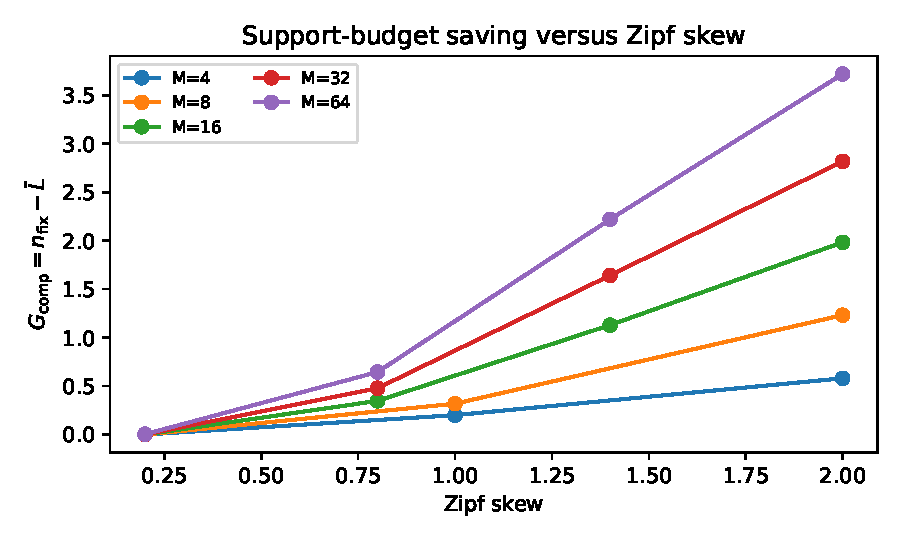
\includegraphics[width=0.86\linewidth,height=0.25\textheight,keepaspectratio]{figures/source_support_saving_vs_zipf.pdf}
\caption{Source-dependent average support-index allocation. This diagnostic reports a classical length-derived coordinate.}\label{fig:secondary-source_support_saving_vs_zipf}
\end{figure}
\begin{figure}[p]\centering
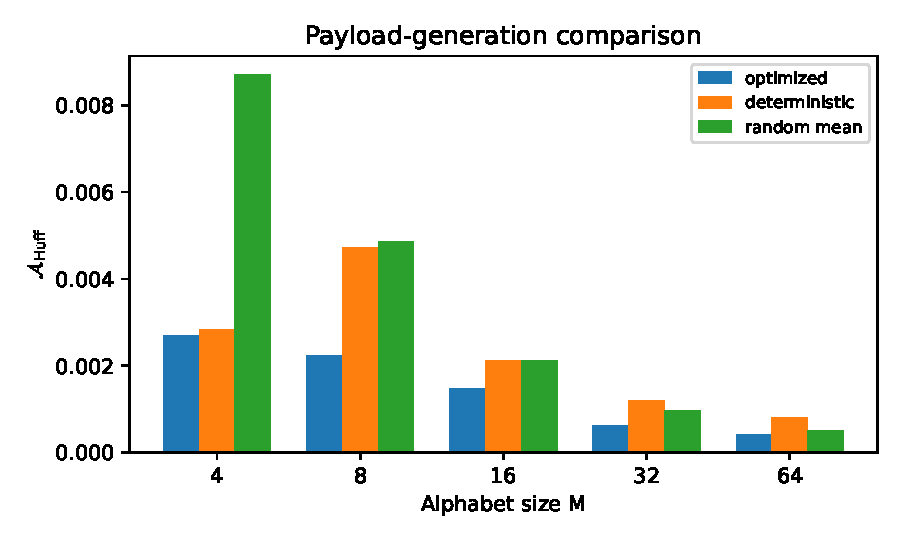
\includegraphics[width=0.86\linewidth,height=0.25\textheight,keepaspectratio]{figures/payload_generation_comparison.pdf}
\caption{Secondary payload-generation comparison with the original deterministic, random-phase, and local-search modes.}\label{fig:secondary-payload_generation_comparison}
\end{figure}
\begin{figure}[p]\centering
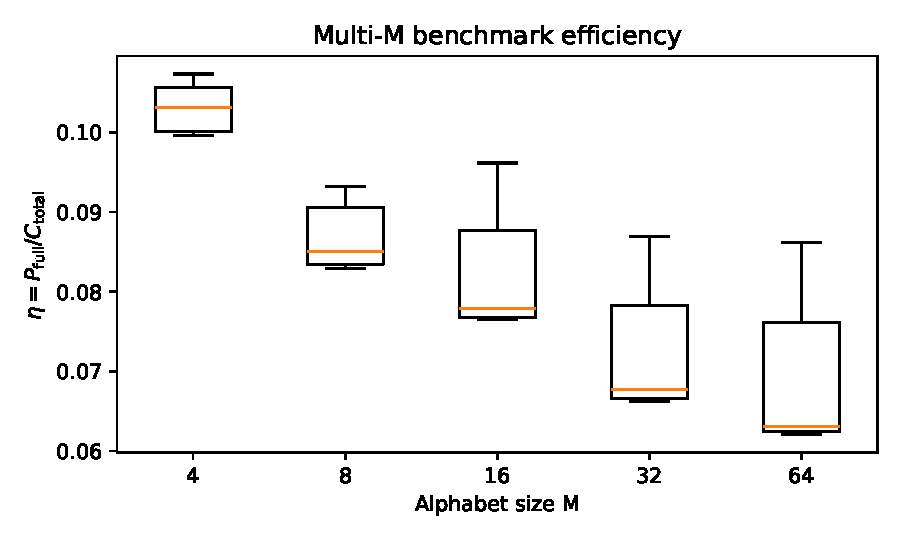
\includegraphics[width=0.86\linewidth,height=0.25\textheight,keepaspectratio]{figures/multiM_benchmark_efficiency.pdf}
\caption{Scalable PGM efficiency benchmark under the declared scalarized cost convention.}\label{fig:secondary-multiM_benchmark_efficiency}
\end{figure}
\begin{figure}[p]\centering
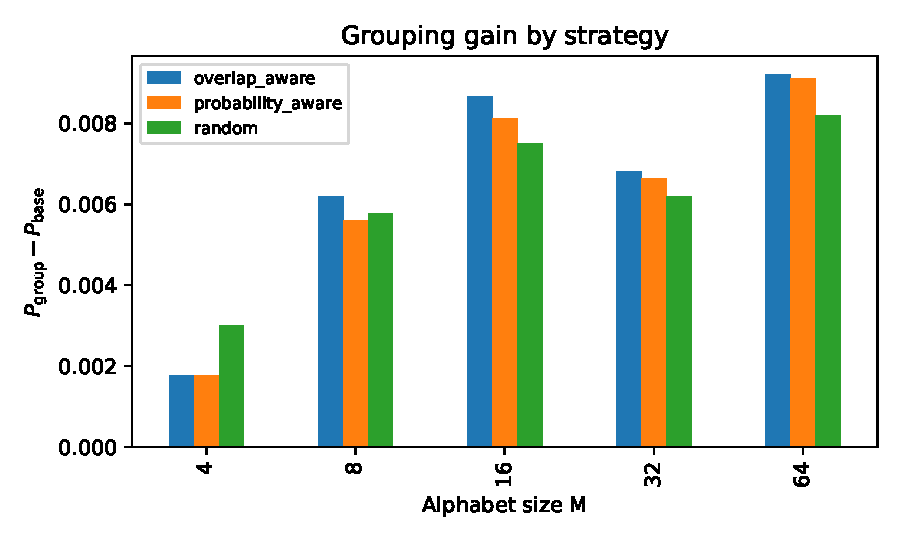
\includegraphics[width=0.86\linewidth,height=0.25\textheight,keepaspectratio]{figures/grouping_gain_by_strategy.pdf}
\caption{Secondary grouping comparison. Overlap-aware grouping is a geometry-dependent heuristic, outside the registered main comparison.}\label{fig:secondary-grouping_gain_by_strategy}
\end{figure}
\begin{figure}[p]\centering
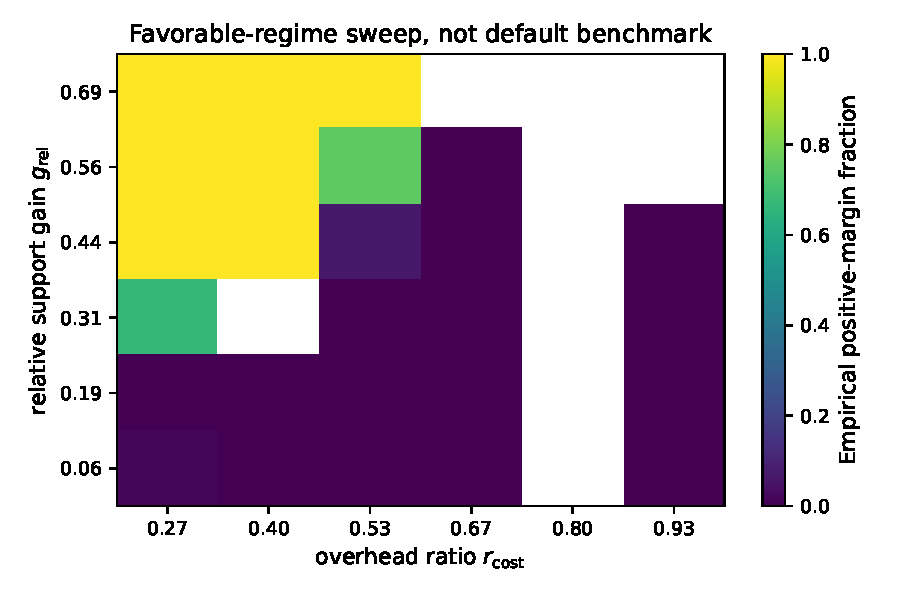
\includegraphics[width=0.86\linewidth,height=0.25\textheight,keepaspectratio]{figures/favorable_sweep_heatmap.pdf}
\caption{Finite sampled favorable-regime PGM diagnostic; the color scale is a convention-dependent scalar margin.}\label{fig:secondary-favorable_sweep_heatmap}
\end{figure}
\begin{figure}[p]\centering
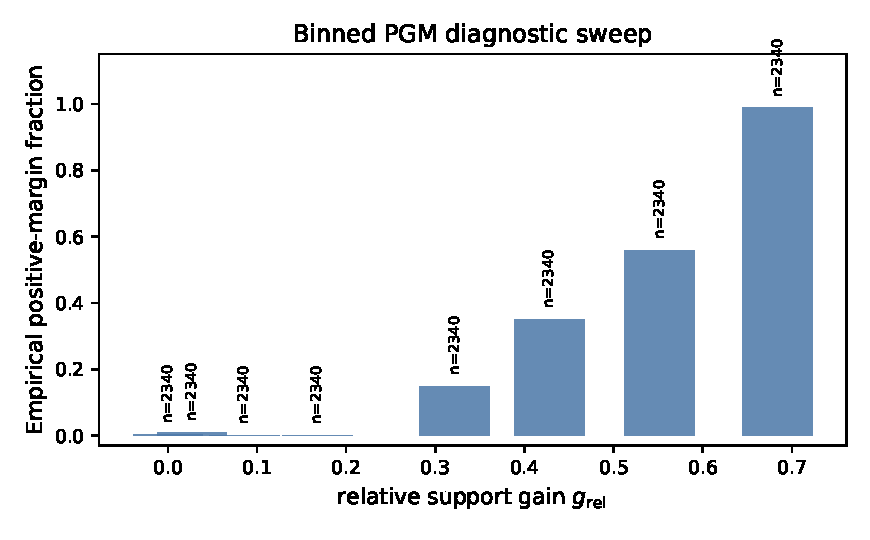
\includegraphics[width=0.86\linewidth,height=0.25\textheight,keepaspectratio]{figures/favorable_positive_fraction_vs_grel.pdf}
\caption{Finite sampled favorable-regime diagnostic versus relative support-index saving. Fractions describe sampled design rows.}\label{fig:secondary-favorable_positive_fraction_vs_grel}
\end{figure}
\begin{figure}[p]\centering
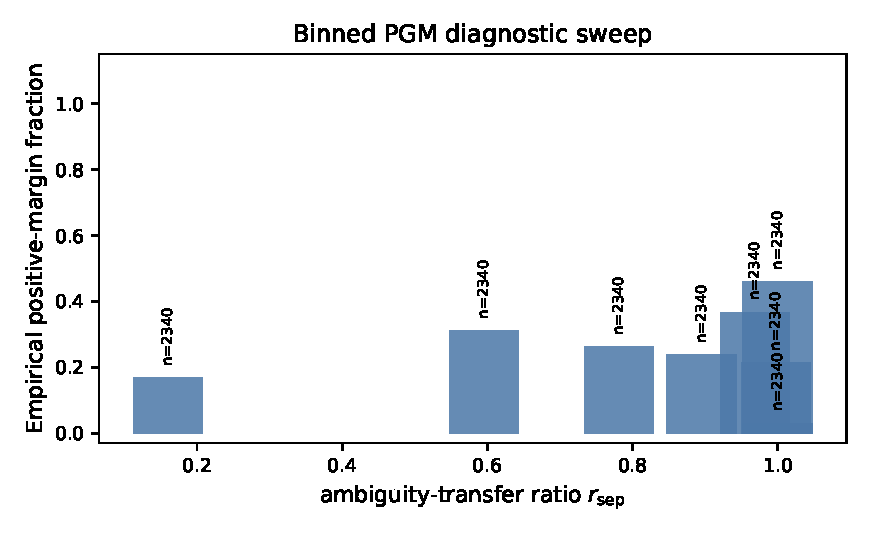
\includegraphics[width=0.86\linewidth,height=0.25\textheight,keepaspectratio]{figures/favorable_positive_fraction_vs_rsep.pdf}
\caption{Finite sampled favorable-regime diagnostic versus removed overlap ambiguity.}\label{fig:secondary-favorable_positive_fraction_vs_rsep}
\end{figure}
\begin{figure}[p]\centering
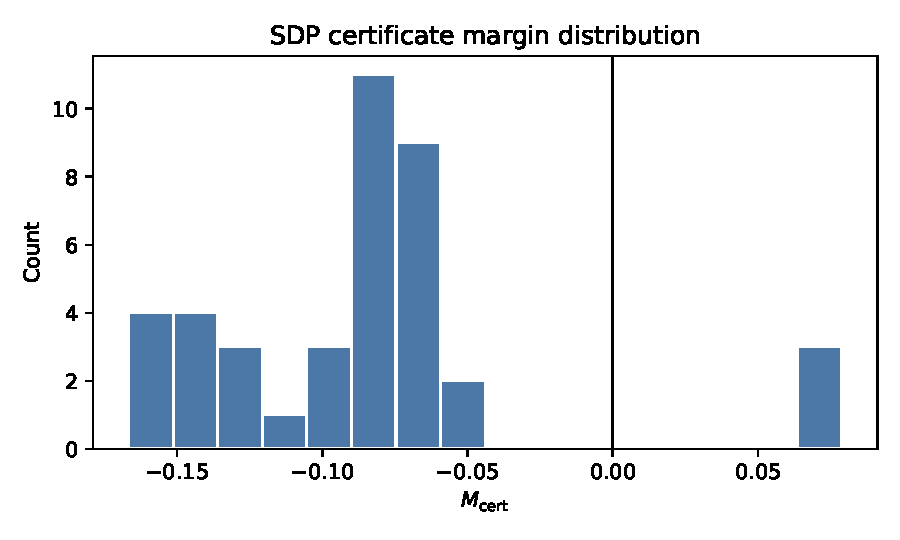
\includegraphics[width=0.86\linewidth,height=0.25\textheight,keepaspectratio]{figures/M_cert_distribution.pdf}
\caption{Secondary small-instance scalarized certificate margins. The fixed reference and accounting differ from the side-information-matched main comparison.}\label{fig:secondary-M_cert_distribution}
\end{figure}
\begin{figure}[p]\centering
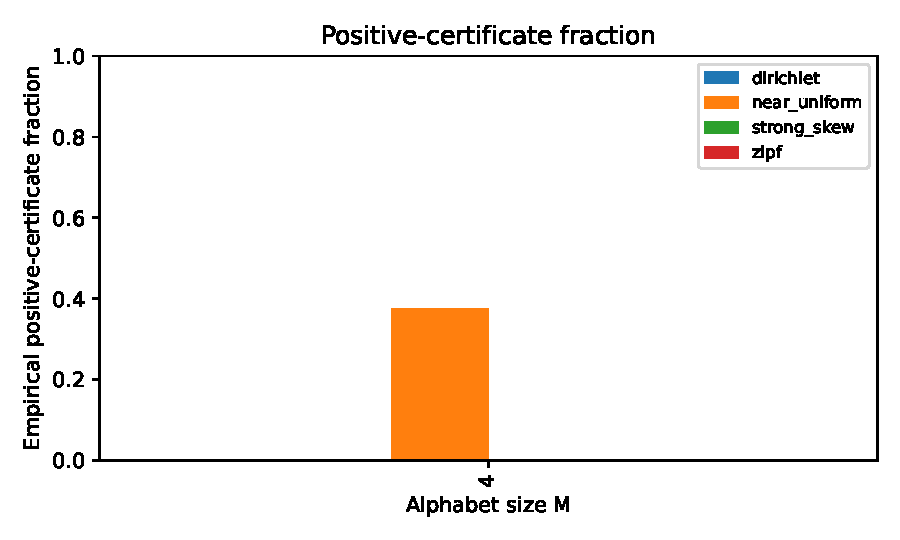
\includegraphics[width=0.86\linewidth,height=0.25\textheight,keepaspectratio]{figures/positive_certificate_ratio.pdf}
\caption{Secondary scalarized certificate fraction for the original finite sample; PGM rows are diagnostics.}\label{fig:secondary-positive_certificate_ratio}
\end{figure}
\begin{figure}[p]\centering
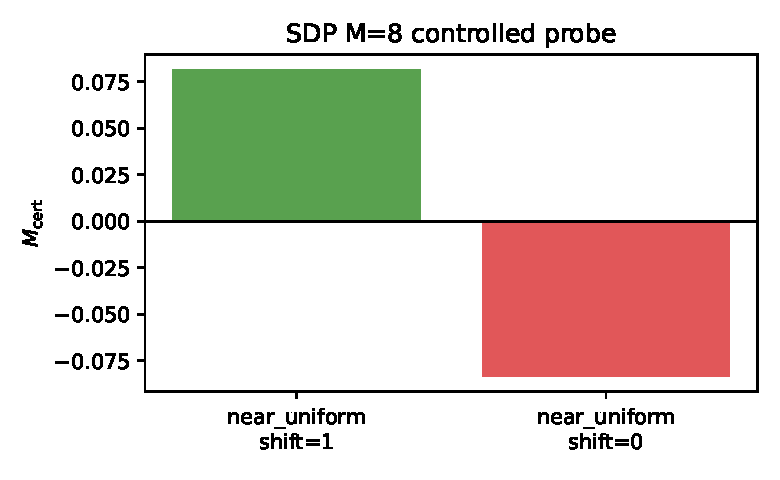
\includegraphics[width=0.86\linewidth,height=0.25\textheight,keepaspectratio]{figures/exact_sdp_m8_probe.pdf}
\caption{Two controlled secondary M=8 scalarized SDP certificate probes, distinct from the registered matched family.}\label{fig:secondary-exact_sdp_m8_probe}
\end{figure}
\begin{figure}[p]\centering
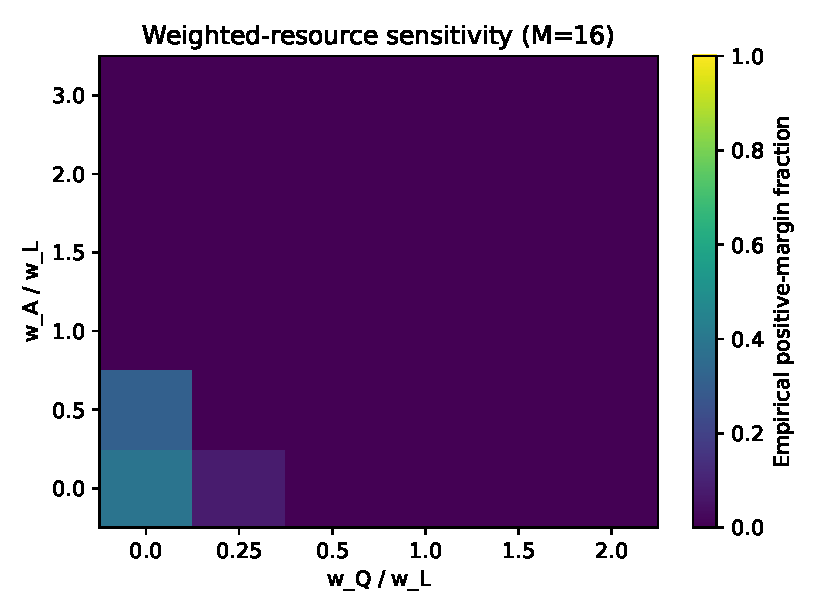
\includegraphics[width=0.86\linewidth,height=0.25\textheight,keepaspectratio]{figures/weighted_resource_sensitivity_heatmap.pdf}
\caption{Weighted scalarized resource sensitivity. The weights are declared comparison conventions rather than hardware calibration.}\label{fig:secondary-weighted_resource_sensitivity_heatmap}
\end{figure}
\begin{figure}[p]\centering
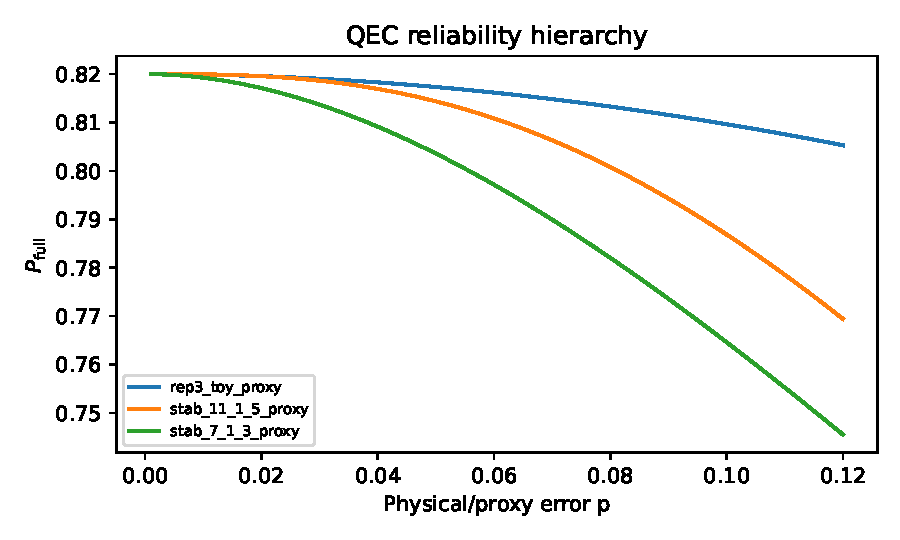
\includegraphics[width=0.86\linewidth,height=0.25\textheight,keepaspectratio]{figures/qec_reliability_hierarchy.pdf}
\caption{Effective logical-failure toy and proxy reliability diagnostics.}\label{fig:secondary-qec_reliability_hierarchy}
\end{figure}

\FloatBarrier
\bibliographystyle{apsrev4-2}
\bibliography{references}
\end{document}
